\باب{برقرار برقی طاقت}

\حصہ{لمحاتی طاقت}
شکل \حوالہ{شکل_طاقت_پرزے_کو_منتقل} میں بوجھ \عددی{\bZ} کو بدلتی رو منبع  طاقت فراہم کرتا ہے۔اس عمومی دور کے برقرار دباو اور برقرار رو درج ذیل لکھے جا سکتے ہیں۔
\begin{gather}
\begin{aligned}\label{مساوات_طاقت_دباو_رو_عمومی_الف}
v(t)&=V_0\cos(\omega t +\theta_v)\\
i(t)&=I_0\cos(\omega t +\theta_i)
\end{aligned}
\end{gather}
یوں کسی بھی لمحہ بوجھ کو منتقل طاقت درج ذیل ہو گا
\begin{gather}
\begin{aligned}
p(t)&=v(t)i(t)\\
&=V_0 I_0  \cos(\omega t +\theta_v) \cos(\omega t +\theta_i)
\end{aligned}
\end{gather}
جس میں
\begin{align}
\cos \alpha \cos \beta=\frac{\cos(\alpha-\beta)+\cos(\alpha+\beta)}{2}
\end{align}
استعمال کرتے ہوئے
\begin{align}\label{مساوات_طاقت_لمحاتی_طاقت_الف}
p(t)=\frac{V_0 I_0}{2}\left[\cos(\theta_v-\theta_i)+\cos(2\omega t +\theta_v+\theta_i)\right]
\end{align}
ملتا ہے جہاں \عددی{\alpha=\omega t +\theta_v} اور \عددی{\beta=\omega t+\theta_i} لئے گئے ہیں۔آپ دیکھ سکتے ہیں کہ لمحاتی طاقت دو اجزاء کا مجموعہ ہے۔پہلا جزو مستقل طاقت ہے جو وقت کے ساتھ تبدیل نہیں ہوتا جبکہ دوسرا جزو دگنی تعدد کا بدلتی رو طاقت ہے۔  
%
\begin{figure}
\centering
\begin{tikzpicture}
\draw(0,0) to [american voltage source,l={$v(t)$}]++(0,\y) to [short,i={$i(t)$}]++(\x,0) to [european resistor,l={$\bZ$}]++(0,-\y) to [short](0,0);
\end{tikzpicture}
\caption{بدلتی رو دور۔}
\label{شکل_طاقت_پرزے_کو_منتقل}
\end{figure}
%======================
\ابتدا{مثال}\شناخت{مثال_طاقت_عمومی_الف}
شکل \حوالہ{شکل_طاقت_پرزے_کو_منتقل} میں برقرار دباو \عددی{v(t)=15\cos(100 t+45^{\circ})\,\si{\volt}} اور \عددی{\bZ=5\phase{20^{\circ}}\,\si{\ohm}} ہیں۔بوجھ کو منتقل لمحاتی طاقت دریافت کریں۔

حل:دوری سمتیات استعمال کرتے ہوئے
\begin{align*}
\hat{I}&=\frac{15\phase{45^{\circ}}}{5\phase{20^{\circ}}}\\
&=3\phase{25^{\circ}}\,\si{\ampere}
\end{align*}
یعنی
\begin{align*}
i(t)=3\cos(100 t +25^{\circ}) \, \si{\ampere}
\end{align*}
لکھا جا سکتا ہے۔یوں مساوات \حوالہ{مساوات_طاقت_لمحاتی_طاقت_الف} سے لمحاتی طاقت درج ذیل لکھی جا سکتی ہے۔
 \begin{align*}
p(t)&=22.5\left[\cos 20^{\circ}+\cos(200 t +70^{\circ})\right] \\
&=21.143+22.5\cos(200t+70^{\circ})\,\si{\watt}
\end{align*}
دباو، رو اور طاقت کے خط شکل \حوالہ{شکل_طاقت_عمومی_الف} میں دکھائے گئے ہیں۔درج بالا مساوات میں \عددی{\SI{21.143}{\watt}} مستقل طاقت ہے جو وقت کے ساتھ تبدیل نہیں ہوتا جبکہ \عددی{22.5\cos(200t+70^{\circ})\,\si{\watt}} بدلتی رو طاقت ہے جس کی تعدد \عددی{\SI{200}{\radian\per\second}} ہے۔
\begin{figure}
\centering
\begin{subfigure}{0.5\textwidth}
\centering
\begin{tikzpicture}
\begin{axis}[kStyleCircuitsA,small,xlabel=$\omega t$, xtick={90,180,270,360},xticklabels={$90^{\circ}$,$180^{\circ}$,$270^{\circ}$,$360^{\circ}$},]
\addplot[domain=0:370,samples=100]{15*cos(1*x+45)}node[pos=0.7,left]{$v(t)$};
\addplot[domain=0:370,samples=100]{3*cos(1*x+25)}node[pos=0.9,above]{$i(t)$};
\end{axis}%
\end{tikzpicture}%
\end{subfigure}%
\begin{subfigure}{0.5\textwidth}
\centering
\begin{tikzpicture}
\begin{axis}[kStyleCircuitsA,small,xlabel=$\omega t$, xtick={90,180,270,360},xticklabels={$90^{\circ}$,$180^{\circ}$,$270^{\circ}$,$360^{\circ}$},]
\addplot[domain=0:370,samples=100]{21.143+22.5*cos(2*x+25)}node[pos=0.4,left]{$p(t)$};
\end{axis}%
\end{tikzpicture}%
\end{subfigure}%
\caption{مثال \حوالہ{مثال_طاقت_عمومی_الف} کے اشکال۔}
\label{شکل_طاقت_عمومی_الف}
\end{figure}
\انتہا{مثال}
%==============
\ابتدا{مثال}
شکل \حوالہ{شکل_طاقت_پرزے_کو_منتقل} میں \عددی{v(t)=V_0\cos(\omega t +\theta_v)\,\si{\volt}} اور \عددی{\bZ=Z_0\phase{\theta_z}\,\si{\ohm}} ہیں۔رو دریافت کریں۔

حل:دوری سمتیات استعمال کرتے ہوئے
\begin{align*}
\hat{I}&=\frac{V_0\phase{\theta_v}}{Z_0\phase{\theta_z}}\\
&=\frac{V_0}{Z_0}\phase{\theta_v-\theta_z}
\end{align*}
لکھا جا سکتا ہے جس سے وقتی دائرہ کار میں رو درج ذیل حاصل ہوتی ہے۔
\begin{align}
i(t)=\frac{V_0}{Z_0} \cos(\omega t+\theta_v-\theta_z)
\end{align}
مساوات \حوالہ{مساوات_طاقت_دباو_رو_عمومی_الف} میں دیے عمومی رو کے ساتھ موازنہ کرتے ہوئے آپ دیکھ سکتے ہیں کہ \عددی{\theta_i} درحقیقت میں \عددی{\theta_v-\theta_z} کے برابر ہے  جسے درج ذیل لکھا جا سکتا ہے۔
\begin{align}\label{مساوات_طاقت_زاویہ_رکاوٹ_اور_طاقت}
\theta_v-\theta_i=\theta_z
\end{align}
\انتہا{مثال}
%=====================

\حصہ{اوسط طاقت}
دہراتے تفاعل (مثلاً سائن نما تفاعل) کے ایک دوری عرصے پر تکمل کو دوری عرصے سے تقسیم کرنے سے تفاعل کی اوسط قیمت حاصل ہوتی ہے۔یوں مساوات \حوالہ{مساوات_طاقت_دباو_رو_عمومی_الف} میں دیے دباو اور رو کی صورت میں بوجھ کو منتقل اوسط طاقت درج ذیل ہو گی
\begin{gather}
\begin{aligned}\label{مساوات_طاقت_اوسط_تکمل_الف}
P&=\frac{1}{T}\int_{t_0}^{t_0+T} p(t) \dif t\\
&=\frac{V_0 I_0}{T}\int_{t_0}^{t_0+T} \cos(\omega t +\theta_v) \cos(\omega t +\theta_i) \dif t
\end{aligned}
\end{gather}    
جہاں \عددی{t_0} کوئی بھی لمحہ ہو سکتا ہے جبکہ \عددی{T=\tfrac{2\pi}{\omega}} دباو یا رو کا دوری عرصہ ہے۔حقیقت میں ہم ایک دوری عرصے کی بجائے  \عددی{n} مکمل دوری عرصے پر تکمل لیتے ہوئے \عددی{n} دوری عرصے سے تقسیم کرتے ہوئے بھی اوسط قیمت حاصل کر سکتے ہیں۔یوں اوسط طاقت درج ذیل بھی لکھی جا سکتی ہے۔
\begin{align}
P&=\frac{V_0 I_0}{nT}\int_{t_0}^{t_0+nT} \cos(\omega t +\theta_v) \cos(\omega t +\theta_i) \dif t
\end{align} 
مساوات \حوالہ{مساوات_طاقت_لمحاتی_طاقت_الف} کی مدد سے مساوات \حوالہ{مساوات_طاقت_اوسط_تکمل_الف} درج ذیل لکھا جائے گا۔
\begin{gather}
\begin{aligned}\label{مساوات_طاقت_اوسط_تکمل_ب}
P&=\frac{V_0 I_0}{2T}\int_{t_0}^{t_0+T} \left[\cos(\theta_v-\theta_i)+\cos(2\omega t +\theta_v+\theta_i)\right] \dif t\\
&=\frac{V_0 I_0}{2T}\int_{t_0}^{t_0+T} \cos(\theta_v-\theta_i) \dif t+\frac{V_0 I_0}{2T}\int_{t_0}^{t_0+T} \cos(2\omega t +\theta_v+\theta_i)\dif t
\end{aligned}
\end{gather} 
درج بالا تکمل کے دو اجزاء کو باری باری حل کرتے ہیں۔پہلا جزو مستقل ہے لہٰذا اس کو تکمل کے باہر لکھتے ہوئے حل کرتے ہیں۔
\begin{align*}
\frac{V_0 I_0}{2T}\int_{t_0}^{t_0+T} \cos(\theta_v-\theta_i) \dif t&=\frac{V_0 I_0}{2T}\cos(\theta_v-\theta_i) \int_{t_0}^{t_0+T} \dif t\\
&=\left. \frac{V_0 I_0}{2T}\cos(\theta_v-\theta_i) t\right|_{t_0}^{t_0+T}\\
&=\frac{V_0 I_0}{2}\cos(\theta_v-\theta_i)
\end{align*}
اب مساوات \حوالہ{مساوات_طاقت_اوسط_تکمل_ب} کے دوسرے جزو کو حل کرتے ہیں
\begin{align*}
\frac{V_0 I_0}{2T}\int_{t_0}^{t_0+T} \cos(2\omega t +\theta_v+\theta_i)\dif t&=\left. \frac{V_0 I_0}{2T}\frac{ \sin(2\omega t +\theta_v+\theta_i)}{2\omega}\right|_{t_0}^{t_0+T}\\
&=0
\end{align*}
جہاں \عددی{\sin \alpha=\sin(\alpha+T)} کا استعمال کیا گیا ہے۔یوں مساوات \حوالہ{مساوات_طاقت_اوسط_تکمل_ب} سے درج ذیل اوسط طاقت حاصل  ہوتا ہے۔
\begin{align}\label{مساوات_طاقت_عمومی_الف}
P=\frac{V_0 I_0}{2}\cos(\theta_v-\theta_i)
\end{align}
چونکہ \عددی{\cos(\alpha)=\cos(-\alpha)} کے برابر ہے لہٰذا درج بالا مساوات میں کوسائن کا دلیل \عددی{\theta_v-\theta_i} یا \عددی{\theta_i-\theta_v} لکھا جا سکتا ہے۔مساوات \حوالہ{مساوات_طاقت_زاویہ_رکاوٹ_اور_طاقت} کو استعمال کرتے ہوئے درج بالا مساوات کو دوبارہ لکھتے ہیں۔
\begin{align}\label{مساوات_طاقت_عمومی_ب}
P=\frac{V_0 I_0}{2}\cos \theta_z
\end{align}
خالص مزاحمتی رکاوٹ \عددی{\bZ=R\phase{0^{\circ}}} کا زاویہ ہٹاو \عددی{0^{\circ}} ہوتا ہے لہٰذا \عددی{\cos 0^{\circ}=1} لیتے ہوئے مزاحمتی بوجھ کا طاقت
\begin{align}\label{مساوات_طاقت_مزاحمتی_طاقت_الف}
P_{\text{مزاحمتی}}=\frac{V_0 I_0}{2}
\end{align}
ہو گا جہاں \عددی{V_0} سے مراد مزاحمت کے دباو کا حیطہ ہے۔قانون اوہم سے درج بالا کو درج ذیل صورتوں میں بھی لکھا جا سکتا ہے۔
\begin{align}
P_{\text{مزاحمتی}}&=\frac{I^2_0 R}{2} \label{مساوات_طاقت_مزاحمتی_طاقت_ب}\\
P_{\text{مزاحمتی}}&=\frac{V^2_0}{2 R} \label{مساوات_طاقت_مزاحمتی_طاقت_پ}
\end{align}
درج بالا تینوں مساوات کا یک سمتی رو میں مزاحمتی ضیاع کے مساوات کے ساتھ موازنہ کرنے سے معلوم ہوتا ہے کہ موجودہ تینوں مساوات کے نسب نما میں دو \عددی{(2)} کا اضافی عدد پایا جاتا ہے جس پر حصہ \حوالہ{حصہ_طاقت_موثر_قیمت} میں  تبصرہ کیا جائے گا۔

امالی متعاملیت کی رکاوٹ \عددی{\bZ_L=X_L\phase{90^{\circ}}} جبکہ برق گیر متعاملیت کی رکاوٹ \عددی{\bZ_C=X_C\phase{-90^{\circ}}} ہوتی ہے۔چونکہ \عددی{\cos (\mp 90^{\circ})=0} ہوتا ہے لہٰذا غیر مزاحمتی رکاوٹ کی طاقت صفر ہو گی۔
\begin{align}
P_{\text{متعاملی}} =0
\end{align}
چونکہ خالص متعامل پرزوں کو صفر اوسط طاقت منتقل ہوتی ہے لہٰذا انہیں \اصطلاح{بے ضیاع پرزے}\فرہنگ{بے ضیاع پرزے}\حاشیہب{lossless components}\فرہنگ{lossless components} کہتے ہیں۔دور کا متعامل حصہ، دوری عرصے کے کچھ حصے میں  دور سے طاقت حاصل کرتے ہوئے  ذخیرہ کرتا ہے  جبکہ دوری عرصے کے کسی دوسرے حصے میں اسی طاقت کو دور کو واپس کرتا ہے۔

%==========================
\ابتدا{مثال}\شناخت{مثال_طاقت_مزاحمت_امالہ_الف}
شکل \حوالہ{مشق_طاقت_مزاحمت_امالہ_الف} میں رکاوٹ کی اوسط طاقت دریافت کریں۔
\begin{figure}
\centering
\begin{tikzpicture}
\draw(0,0) to [american voltage source,l={$50\phase{30^{\circ}}\,\si{\volt}$}]++(0,2*\y) to [short,i={$\hat{I}$}]++(\x,0) to [resistor,l={$\SI{3}{\ohm}$}]++(0,-\y) to [inductor,l={$j6 \,\si{\ohm}$}]++(0,-\y) to [short] (0,0);
\end{tikzpicture}
\caption{مثال \حوالہ{مثال_طاقت_مزاحمت_امالہ_الف} کا دور۔}
\label{مشق_طاقت_مزاحمت_امالہ_الف}
\end{figure}

حل:رو درج ذیل ہے۔
\begin{align*}
\hat{I}&=\frac{50\phase{30^{\circ}}}{3+j6}=\frac{50\phase{30^{\circ}}}{3+j6}=\frac{50\phase{30^{\circ}}}{\sqrt{45}\phase{63.435^{\circ}}}=7.454\phase{-33.435^{\circ}}\,\si{\ampere}
\end{align*}
یوں
\begin{align*}
P&=\frac{V_0 I_0}{2}\cos(\theta_v-\theta_i)\\
&=\frac{(50)(7.454)}{2}\cos[30^{\circ}-(-33.435^{\circ})]\\
&=\SI{83.34}{\watt}
\end{align*}
ہو گا۔چونکہ طاقت صرف مزاحمت میں ضائع ہوتی ہے لہٰذا یہی جواب مساوات \حوالہ{مساوات_طاقت_مزاحمتی_طاقت_الف} سے بھی حاصل کیا جا سکتا ہے جہاں \عددی{V_0} سے مراد مزاحمت کے دباو کا حیطہ ہے۔تقسیم دباو سے مزاحمت کا دباو درج ذیل ہے
\begin{align*}
\hat{V}_R&=\left(\frac{3}{3+j6}\right)50\phase{30^{\circ}}=22.361\phase{-33.435^{\circ}}
\end{align*}
جس سے مزاحمت کا اوسط طاقت درج ذیل ہو گا۔
\begin{align*}
P&=\frac{V_0 I_0}{2}=\frac{(22.361)(7.454)}{2}=\SI{83.34}{\watt}
\end{align*}
اسی طرح مساوات \حوالہ{مساوات_طاقت_مزاحمتی_طاقت_ب} اور مساوات \حوالہ{مساوات_طاقت_مزاحمتی_طاقت_پ} بھی استعمال کیے جا سکتے ہیں
\begin{align*}
P&=\frac{I^2_0 R}{2}=\frac{(7.454^2)(3)}{2}=\SI{83.34}{\watt}\\
P&=\frac{V^2_0}{2 R}=\frac{(22.361^2)}{(2)(3)}=\SI{83.34}{\watt}
\end{align*}
\انتہا{مثال}
%==========================
\ابتدا{مثال}\شناخت{مثال_طاقت_مزاحمت_امالہ_ب}
شکل \حوالہ{شکل_طاقت_مزاحمت_امالہ_ب} میں منبع دباو کا اوسط طاقت حاصل کریں۔دور کے بقایا پرزوں کا اوسط طاقت بھی دریافت کریں۔
\begin{figure}
\centering
\begin{tikzpicture}
\draw(0,0) to [american voltage source,i^<={$\hat{I}_m$},l={$10\phase{30^{\circ}}\,\si{\volt}$}]++(0,2*\y) to [short]++(4*\x,0) to [capacitor,i>_={$\hat{I}_C$},l={$-j10\,\si{\ohm}$}]++(0,-2*\y) to [short] (0,0);
\draw(\x,0) to [inductor,i_<={$\hat{I}_L$},*-*,l={$j5\,\si{\ohm}$}]++(0,2*\y);
\draw(2*\x,0) to [resistor,i_<={$\hat{I}_R$},*-*,l={$\SI{2}{\ohm}$}]++(0,2*\y);
\draw(3*\x,0) to [inductor,*-,l={$j2\,\si{\ohm}$}]++(0,\y) to [resistor,i_<={$\hat{I}_Z$},-*,l={$\SI{2}{\ohm}$}]++(0,\y);
\end{tikzpicture}
\caption{مثال \حوالہ{مثال_طاقت_مزاحمت_امالہ_ب} کا دور۔}
\label{شکل_طاقت_مزاحمت_امالہ_ب}
\end{figure} 

حل:پہلے تمام رو دریافت کرتے ہیں۔شکل میں دباو کو دیکھتے ہوئے انفعالی رائج رو کے تحت رو کی سمتیں چننی گئی ہیں۔ 
\begin{align*}
\hat{I}_L&=\frac{10\phase{30^{\circ}}}{j5}=\frac{10\phase{30^{\circ}}}{5\phase{90^{\circ}}}=2\phase{-60^{\circ}}\\
\hat{I}_R&=\frac{10\phase{30^{\circ}}}{2}=\frac{10\phase{30^{\circ}}}{2\phase{0^{\circ}}}=5\phase{30^{\circ}}\\
\hat{I}_Z&=\frac{10\phase{30^{\circ}}}{2+j2}=\frac{10\phase{30^{\circ}}}{\sqrt{8}\phase{45^{\circ}}}=\frac{5}{\sqrt{2}}\phase{-15^{\circ}}\\
\hat{I}_C&=\frac{10\phase{30^{\circ}}}{-j10}=\frac{10\phase{30^{\circ}}}{10\phase{-90^{\circ}}}=1\phase{120^{\circ}}\\
\hat{I}_m&=-\left[\hat{I}_L+\hat{I}_R+\hat{I}_Z+\hat{I}_C\right]=8.27647\phase{-175.01689^{\circ}}
\end{align*}
یوں انفرادی شاخوں کے اوسط طاقت مساوات \حوالہ{مساوات_طاقت_عمومی_الف} یا مساوات \حوالہ{مساوات_طاقت_عمومی_ب} سے درج ذیل ہوں گے۔
\begin{align*}
P_L&=\frac{(30)(2)}{2}\cos(90^{\circ})&=\SI{0}{\watt}\\
P_R&=\frac{(30)(5)}{2}\cos(0^{\circ})&=\SI{75}{\watt}\\
P_Z&=\frac{(30)(\tfrac{5}{\sqrt{2}})}{2}\cos(45^{\circ})&=\SI{37.5}{\watt}\\
P_C&=\frac{(30)(1)}{2}\cos(90^{\circ})&=\SI{0}{\watt}\\
P_m&=\frac{(30)(8.27647)}{2}\cos[(30^{\circ}+175.01689^{\circ})]&=-\SI{112.5}{\watt}
\end{align*}
مثبت جواب طاقت کا ضیاع ہے جبکہ منفی جواب طاقت کی پیداوار ہے۔آپ دیکھ سکتے ہیں کہ منبع کی طاقتی پیداوار \عددی{\SI{112.5}{\watt}} ہے جو دور میں طاقت کے ضیاع 
\begin{align*}
P_L+P_R+P_Z+P_C=0+75+37.5+0=\SI{112.5}{\watt}
\end{align*}
کے عین برابر ہے۔
\انتہا{مثال}
%==========================
\ابتدا{مشق}\شناخت{مشق_طاقت_دریافت_کریں_الف}
شکل \حوالہ{شکل_طاقت_دریافت_کریں_الف} کے تمام مزاحمتوں میں ضائع ہونے والا اوسط طاقت دریافت کریں۔


\begin{figure}
\centering
\begin{tikzpicture}
\draw(0,0) to [american voltage source,l={$22\phase{-30^{\circ}}\,\si{\volt}$}]++(0,2*\y) to [capacitor,l={$-j2\,\si{\ohm}$}]++(\x,0) to [resistor,l={$\SI{4}{\ohm}$}]++(\x,0) to [inductor,l={$j1\,\si{\ohm}$}]++(0,-\y) to [resistor,l={$\SI{5}{\ohm}$}]++(0,-\y) to [short] (0,0);
\draw(2*\x,2*\y) to [short,*-]++(\x,0) to [inductor,l={$j10\,\si{\ohm}$}]++(0,-2*\y) to [short,-*]++(-\x,0);
\end{tikzpicture}
\caption{مشق \حوالہ{مشق_طاقت_دریافت_کریں_الف} کا دور۔}
\label{شکل_طاقت_دریافت_کریں_الف}
\end{figure}

جوابات:\عددی{P_{\SI{4}{\ohm}}=\SI{17.491}{\watt}}، \عددی{P_{\SI{5}{\ohm}}=\SI{14.975}{\watt}}
\انتہا{مشق}
%============================

%==========================
\ابتدا{مشق}\شناخت{مشق_طاقت_دریافت_کریں_ب}
شکل \حوالہ{شکل_طاقت_دریافت_کریں_ب} کے تمام مزاحمتوں میں ضائع ہونے والا اوسط طاقت دریافت کریں۔
\begin{figure}
\centering
\begin{tikzpicture}
\draw(0,0) to [american current source,l={$10\phase{45^{\circ}}\,\si{\ampere}$}]++(0,\yy) to [capacitor,l={$-j2\,\si{\ohm}$}]++(\xx,0) to [resistor,l={$\SI{4}{\ohm}$}]++(0,-\yy) to [short] (0,0);
\draw(0,\yy) to [resistor,*-,l_={$\SI{2}{\ohm}$}]++(-\xx,0) to [inductor,l_={$j4\,\si{\ohm}$}]++(0,-\yy) to [short,-*] (0,0);
\end{tikzpicture}
\caption{مشق \حوالہ{مشق_طاقت_دریافت_کریں_ب} کا دور۔}
\label{شکل_طاقت_دریافت_کریں_ب}
\end{figure}

جوابات:\عددی{P_{\SI{2}{\ohm}}=\SI{50}{\watt}}، \عددی{P_{\SI{4}{\ohm}}=\SI{100}{\watt}}
\انتہا{مشق}
%====================
\ابتدا{مشق}\شناخت{مشق_طاقت_دریافت_کریں_پ}
شکل \حوالہ{شکل_طاقت_دریافت_کریں_پ} کے تمام مزاحمتوں میں ضائع ہونے والا اوسط طاقت دریافت کریں۔
\begin{figure}
\centering
\begin{tikzpicture}
\draw(0,0) to [american voltage source,l={$20\phase{30^{\circ}}\,\si{\volt}$}]++(0,\yy) to [european resistor,l={$2+j2\,\si{\ohm}$}]++(\xx,0) to [european resistor,l={$6+j2\,\si{\ohm}$}]++(0,-\yy) to [short] (0,0);
\draw(\xx,0) to [short,*-]++(\xx,0) to [american voltage source,l_={$40\phase{60^{\circ}}\,\si{\volt}$}]++(0,\yy) to [european resistor,l_={$3-j4\,\si{\ohm}$},-*]++(-\xx,0);
\end{tikzpicture}
\caption{مشق \حوالہ{مشق_طاقت_دریافت_کریں_پ} کا دور۔}
\label{شکل_طاقت_دریافت_کریں_پ}
\end{figure}

جوابات:\عددی{P_{\SI{2}{\ohm}}=\SI{22.72}{\watt}} ،\عددی{P_{\SI{3}{\ohm}}=\SI{5.71}{\watt}}، \عددی{P_{\SI{6}{\ohm}}=\SI{11.42}{\watt}}
\انتہا{مشق}
%==============

ایک سے زیادہ منبع کی صورت میں آپ کسی بھی ترکیب کو استعمال کرتے ہوئے شاخوں کی رو اور جوڑ کے دباو حاصل کرتے ہوئے طاقت دریافت کر سکتے ہیں۔البتہ یاد رہے کہ ترکیب نفاذ سے طاقت کا تخمینہ نہیں لگایا جا سکتا چونکہ طاقت مربع دباو (یا مربع رو) کا تعلق رکھتا ہے جو غیر خطی تعلق ہے۔ 

%===============
\ابتدا{مشق}\شناخت{مشق_طاقت_دریافت_کریں_ت}
شکل \حوالہ{شکل_طاقت_دریافت_کریں_ت} میں اوسط طاقت کی پیداوار اور ضیاع معلوم کریں۔ 
\begin{figure}
\centering
\begin{tikzpicture}
\draw(0,0) to [american voltage source,l={$20\phase{30^{\circ}}\,\si{\volt}$}]++(0,\y) to [resistor,l={$\SI{2}{\ohm}$}]++(\x,0) to [inductor,l={$j4\,\si{\ohm}$}]++(\x,0);
\draw(0,0) to [short]++(2*\x,0) to [american voltage source,l_={$40\phase{0^{\circ}}\,\si{\volt}$}]++(0,\y);
\end{tikzpicture}
\caption{مشق \حوالہ{مشق_طاقت_دریافت_کریں_ت} کا دور۔}
\label{شکل_طاقت_دریافت_کریں_ت}
\end{figure}

\عددی{P_{20\phase{30^{\circ}}}=\SI{-25.36}{\watt}}، \عددی{P_{40\phase{0^{\circ}}}=\SI{-5.36}{\watt}}، \عددی{P_{\SI{2}{\ohm}}=\SI{30.72}{\watt}}
\انتہا{مشق}
%================

\ابتدا{مشق}\شناخت{مشق_طاقت_دریافت_کریں_ٹ}
شکل \حوالہ{شکل_طاقت_دریافت_کریں_ٹ} میں اوسط طاقت کی پیداوار اور ضیاع معلوم کریں۔ 
\begin{figure}
\centering
\begin{tikzpicture}
\draw(0,0) to [american voltage source,l={$30\phase{0^{\circ}}$}]++(0,\y) to [short]++(\x,0) to [inductor,l={$j8\,\si{\ohm}$}]++(0,-\y) to [short] (0,0);
\draw(\x,0) to [short,*-] ++(\x,0) to [inductor,l_={$j6\,\si{\ohm}$}]++(0,\y) to [capacitor,-*,l_={$-j10\,\si{\ohm}$}]++(-\x,0);
\end{tikzpicture}
\caption{مشق \حوالہ{مشق_طاقت_دریافت_کریں_ٹ} کا دور۔}
\label{شکل_طاقت_دریافت_کریں_ٹ}
\end{figure}

جواب:اوسط طاقت کی پیدا وار اور طاقت کا ضیاع صفر واٹ ہیں۔
\انتہا{مشق}
%================

\حصہ{زیادہ سے زیادہ اوسط طاقت منتقل کرنے کا مسئلہ}
یک سمتی رو ادوار میں ہم زیادہ سے زیادہ طاقت منتقل کرنے کے مسئلے پر ہم حصہ \حوالہ{حصہ_مسئلے_زیادہ_سے_زیادہ_طاقت_منتقل} میں غور کر چکے ہیں۔آئیں بدلتی رو کی صورت میں اسی مسئلے پر دوبارہ غور کریں۔

کسی بھی دور کا تھونن مساوی حاصل کیا جا سکتا ہے۔شکل \حوالہ{شکل_طاقت_زیادہ_سے_زیادہ_الف} میں تھونن مساوی دور کے ساتھ بوجھ جوڑا گیا ہے جہاں تھونن دباو کو \عددی{\hat{V}_{\text{کھلا}}} کہا گیا ہے۔ہم جاننا چاہتے ہیں کہ بوجھ کو کس صورت میں زیادہ سے زیادہ اوسط طاقت منتقل ہو گا۔  
\begin{figure}
\centering
\begin{tikzpicture}[american voltages]
\draw(0,0) to [american voltage source,l={$\hat{V}_{\text{کھلا}}$}]++(0,\y) to [european resistor,l={$\bZ_{\text{تھونن}}$}]++(\x,0) to [short,i={$\hat{I}_{\text{بوجھ}}$}]++(\x,0) to [european resistor,v={$\hat{V}_{\text{بوجھ}}$},l={$\bZ_{\text{تھونن}}$}]++(0,-\y) to [short] (0,0);
\end{tikzpicture}
\caption{زیادہ سے زیادہ اوسط طاقت منتقل کرنے کا مسئلہ۔}
\label{شکل_طاقت_زیادہ_سے_زیادہ_الف}
\end{figure}

شکل کو دیکھ کر درج ذیل لکھا جا سکتا ہے
\begin{align}\label{مساوات_طاقت_زیادہ_سے_زیادہ_طاقت_الف}
\hat{I}_{\text{بوجھ}} &=\frac{\hat{V}_{\text{کھلا}}}{\bZ_{\text{تھونن}}+\bZ_{\text{بوجھ}}}
\end{align}
جہاں
\begin{align*}
\bZ_{\text{تھونن}}&=R_{\text{تھونن}}+jX_{\text{تھونن}}\\
\bZ_{\text{بوجھ}}&=R_{\text{بوجھ}}+jX_{\text{بوجھ}}\\
\hat{V}_{\text{کھلا}}&=V_{\text{کھلا}} \phase{\theta_{\text{کھلا}}}
\end{align*}
ہیں۔درج بالا میں امالی رکاوٹ کی صورت میں \عددی{X} کی قیمت مثبت ہو گی جبکہ برق گیر رکاوٹ کی صورت میں اس کی قیمت منفی ہو گی۔یوں مساوات \حوالہ{مساوات_طاقت_زیادہ_سے_زیادہ_طاقت_الف} کو درج ذیل لکھا جا سکتا ہے
\begin{align*}
\hat{I}_{\text{بوجھ}}&=\frac{V_{\text{کھلا}} \phase{\theta_{\text{کھلا}}}}{R_{\text{تھونن}}+jX_{\text{تھونن}}+R_{\text{بوجھ}}+jX_{\text{بوجھ}}}
\end{align*}
جس کی حتمی قیمت درج ذیل ہے۔
\begin{align*}
I_{\text{بوجھ}}&=\frac{V_{\text{کھلا}}}{\sqrt{(R_{\text{تھونن}}+R_{\text{بوجھ}})^2+(X_{\text{تھونن}}+X_{\text{بوجھ}})^2}}
\end{align*}

بوجھ کو منتقل اوسط طاقت مساوات \حوالہ{مساوات_طاقت_مزاحمتی_طاقت_ب} کی مدد سے لکھتے ہیں۔
\begin{gather}
\begin{aligned}\label{مساوات_طاقت_زیادہ_سے_زیادہ_مساوات_الف}
P_{\text{بوجھ}}&=\frac{1}{2}I^2_{\text{بوجھ}} R_{\text{بوجھ}}\\
&=\frac{\frac{1}{2}V^2_{\text{کھلا}}\, R_{\text{بوجھ}}}{(R_{\text{تھونن}}+R_{\text{بوجھ}})^2+(X_{\text{تھونن}}+X_{\text{بوجھ}})^2}
\end{aligned}
\end{gather} 
ہم جانتے ہیں کہ \عددی{X} میں طاقت ضائع نہیں ہوتا لہٰذا اس کو اوسطاً صفر طاقت منتقل ہوتا ہے۔درج بالا مساوات میں کسر کے نسب نما
 میں \عددی{X_{\text{بوجھ}}+X_{\text{تھونن}}}  کی قیمت کم سے کم کرتے ہوئے طاقت بڑھائی جا سکتی ہے۔درج ذیل صورت میں اس قیمت کو صفر بنایا جا سکتا ہے۔
\begin{align}\label{مساوات_طاقت_زیادہ_سے_زیادہ_مساوات_ب}
X_{\text{بوجھ}}=-X_{\text{تھونن}}  \quad \quad \text{\RL{بوجھ کو زیادہ سے زیادہ طاقت کی منتقلی کا پہلا شرط}}
\end{align}
مساوات \حوالہ{مساوات_طاقت_زیادہ_سے_زیادہ_مساوات_ب} کے شرط پر پورا اترتے ہوئے مساوات \حوالہ{مساوات_طاقت_زیادہ_سے_زیادہ_مساوات_الف} کو درج ذیل لکھا جا سکتا ہے۔
\begin{align}\label{مساوات_طاقت_زیادہ_سے_زیادہ_مساوات_پ}
P_{\text{بوجھ}}&=\frac{V^2_{\text{کھلا}}\, R_{\text{بوجھ}}}{2(R_{\text{تھونن}}+R_{\text{بوجھ}})^2}
\end{align}
آئیں جانتے ہیں کہ کس قیمت کے \عددی{R_{\text{بوجھ}}} کو زیادہ سے زیادہ طاقت  منتقل ہو گی۔یہ جاننے کے لئے درج بالا مساوات کے تفرق کو صفر کے برابر پُر کرتے ہوئے  \عددی{R_{\text{بوجھ}}} کی درکار قیمت حاصل کرتے ہیں۔
\begin{align*}
\frac{\dif P_{\text{بوجھ}}}{\dif R_{\text{بوجھ}}} = \frac{V^2_{\text{بوجھ}}\left(R_{\text{تھونن}}+R_{\text{بوجھ}}\right)^2-2V_{\text{بوجھ}}^2 R_{\text{بوجھ}} \left(R_{\text{تھونن}}+R_{\text{بوجھ}}\right)}{2\left(R_{\text{تھونن}}+R_{\text{بوجھ}}\right)^4} =0
\end{align*}
اس سے
\begin{align}\label{مساوات_طاقت_زیادہ_سے_زیادہ_مساوات_ت}
R_{\text{بوجھ}}=R_{\text{تھونن}} \quad \quad \text{\RL{بوجھ کو زیادہ سے زیادہ طاقت کی منتقلی کا دوسرا شرط}}
\end{align}
حاصل ہوتا ہے۔اس نتیجے کے تحت بوجھ کو اس صورت زیادہ سے زیادہ طاقت منتقل ہو گی جب بوجھ کی مزاحمت دور کے تھونن مزاحمت کے برابر ہو۔مساوات \حوالہ{مساوات_طاقت_زیادہ_سے_زیادہ_مساوات_ب} اور مساوات \حوالہ{مساوات_طاقت_زیادہ_سے_زیادہ_مساوات_ت} کو استعمال کرتے ہوئے، بوجھ کو زیادہ سے زیادہ طاقت منتقل ہونے کی شرط کو درج ذیل لکھا جا سکتا ہے۔
\begin{gather}
\begin{aligned}\label{مساوات_طاقت_بلندتر_شرط_الف}
R_{\text{بوجھ}}+jX_{\text{بوجھ}} &=R_{\text{تھونن}}-jX_{\text{تھونن}}\\
\bZ_{\text{بوجھ}}=\bZ^*_{\text{تھونن}}
\end{aligned}
\end{gather}
مساوات \حوالہ{مساوات_طاقت_بلندتر_شرط_الف} کی صورت میں زیادہ سے زیادہ اوسط طاقت درج ذیل حاصل ہو گی۔
\begin{align}
P_{\text{بلندتر}} = \frac{V^2_{\text{کھلا}}}{8R_{\text{بوجھ}}}
\end{align}
آخر میں یہ بھی بتلاتا چلوں کہ مزاحمتی بوجھ \عددی{(X_L=0)} کی صورت میں مساوات \حوالہ{مساوات_طاقت_زیادہ_سے_زیادہ_مساوات_الف} کے تفرق کو صفر
\begin{align*}
\frac{\dif P_{\text{بوجھ}}}{\dif R_{\text{بوجھ}}}=0
\end{align*}
 کے برابر پر کرنے سے درج ذیل ملتا ہے۔
\begin{align}
R_{\text{بوجھ}}=\sqrt{R^2_{\text{تھونن}}+X^2_{\text{تھونن}}}
\end{align}

%=======================
\ابتدا{مثال}\شناخت{مثال_طاقت_زیادہ_سے-زیادہ_مثال_الف}
شکل \حوالہ{شکل_طاقت_زیادہ_سے-زیادہ_مثال_الف} میں بوجھ کے رکاوٹ کی وہ قیمت دریافت کریں جس پر بوجھ کو زیادہ سے زیادہ طاقت منتقل ہو گا۔اس طاقت کی قیمت بھی دریافت کریں۔
\begin{figure}
\centering
\begin{subfigure}{1\textwidth}
\centering
\begin{tikzpicture}
\draw(0,0) to [american voltage source,l={$20\phase{0^{\circ}}\,\si{\volt}$}]++(0,\y) to [inductor,l={$j2\,\si{\ohm}$}]++(\x,0) to [resistor,l={$\SI{6}{\ohm}$}]++(0,-\y) to [short] (0,0);
\draw(\x,0) to [short,*-]++(\x,0) to [european resistor,l_={$\bZ_{\text{بوجھ}}$}]++(0,\y) to [capacitor,-*,l_={$-j4\,\si{\ohm}$}]++(-\x,0);
\end{tikzpicture}
\caption*{(الف)}
\end{subfigure}
\begin{subfigure}{0.5\textwidth}
\centering
\begin{tikzpicture}
\draw(0,0) to [short]++(0,\y) to [inductor,l={$j2\,\si{\ohm}$}]++(\x,0) to [resistor,l={$\SI{6}{\ohm}$}]++(0,-\y) to [short] (0,0);
\draw(\x,0) to [short,*-o]++(\x,0)++(0,\y) to [capacitor,o-*,l_={$-j4\,\si{\ohm}$}]++(-\x,0);
\draw[stealth-] (2*\x,\y/2)--++(\x/8,0)--++(0,-\y/8)node[below]{$\bZ_{\text{تھونن}}$};
\end{tikzpicture}
\caption*{(ب)}
\end{subfigure}%
\begin{subfigure}{0.5\textwidth}
\centering
\begin{tikzpicture}
\draw(0,0) to [american voltage source,l={$20\phase{0^{\circ}}\,\si{\volt}$}]++(0,\y) to [inductor,l={$j2\,\si{\ohm}$}]++(\x,0) to [resistor,l={$\SI{6}{\ohm}$}]++(0,-\y) to [short] (0,0);
\draw(\x,0) to [short,*-o]++(\x,0) ++(0,\y) to [capacitor,o-*,l_={$-j4\,\si{\ohm}$}]++(-\x,0);
\draw(2*\x,\y/2)node{$\begin{aligned} &+ \\ &\hat{V}_{\text{کھلا}} \\ &- \end{aligned}$};
\end{tikzpicture}
\caption*{(پ)}
\end{subfigure}
\begin{subfigure}{1\textwidth}
\centering
\begin{tikzpicture}
\draw(0,0) to [american voltage source,l={$18.97\phase{-18.43^{\circ}}\,\si{\volt}$}]++(0,\y) to [european resistor,l={${0.6-j2.2\,\si{\ohm}}$}]++(\x,0) to [european resistor,i>^={$\hat{I}_{\text{بوجھ}}$},l={${0.6+j2.2\,\si{\ohm}}$}]++(0,-\y) to [short] (0,0);
\end{tikzpicture}
\caption*{(ت)}
\end{subfigure}
\caption{مثال \حوالہ{مثال_طاقت_زیادہ_سے-زیادہ_مثال_الف} کا دور۔}
\label{شکل_طاقت_زیادہ_سے-زیادہ_مثال_الف}
\end{figure}

حل:سب سے پہلے بوجھ کو ہٹاتے ہوئے بقایا دور کا تھونن مساوی حاصل کرنا ہو گا۔شکل-ب میں منبع دباو کو قصر دور کیا گیا ہے تا کہ تھونن مزاحمت حاصل کی جا سکے۔اسی طرح شکل-پ میں کھلے دور دباو کی نشاندہی کی گئی ہے۔ شکل-ب تھونن رکاوٹ لکھتے ہیں۔
\begin{align*}
\bZ_{\text{تھونن}}&=-j4+\frac{(6)(j2)}{6+j2}=\frac{3}{5}-j\frac{11}{5} \, \si{\ohm}
\end{align*}
یوں بوجھ کو زیادہ سے زیادہ طاقت کی منتقلی کے لئے ضروری ہے کہ بوجھ کی رکاوٹ درج ذیل ہو۔
\begin{align*}
\bZ_{\text{بوجھ}}=\frac{3}{5}+j\frac{11}{5} \, \si{\ohm}
\end{align*} 
شکل-پ میں برق گیر میں صفر رو ہے لہٰذا اس پر دباو بھی صفر ہو گا۔اس طرح مزاحمت پر دباو ہی تھونن دباو ہے جسے تقسیم دباو کے کلیے سے لکھتے ہیں۔
\begin{align*}
\hat{V}_{\text{کھلا}}&=\left(\frac{6}{6+j2}\right) (20\phase{0^{\circ}})=18.97\phase{-18.43^{\circ}}\,\si{\volt}
\end{align*}
شکل-ت میں تھونن مساوی دور کو بوجھ کے ساتھ جوڑ کر دکھایا گیا ہے جہاں سے رو حاصل کرتے ہیں۔
\begin{align*}
\hat{I}_{\text{بوجھ}}&=\frac{18.97\phase{-18.43^{\circ}}}{\frac{3}{5}-j\frac{11}{5}+\frac{3}{5}+j\frac{11}{5}}\\
&=15.81\phase{-18.43^{\circ}}\,\si{\ampere}
\end{align*}
یوں بوجھ کو منتقل اوسط طاقت درج ذیل ہو گا۔
\begin{align*}
P_{\text{بوجھ}}=\frac{(15.81^2)(0.6)}{2}=\SI{74.99}{\watt}
\end{align*}

\انتہا{مثال}
%=================
\ابتدا{مثال}\شناخت{مثال_طاقت_زیادہ_سے-زیادہ_مثال_ب}
شکل \حوالہ{شکل_طاقت_زیادہ_سے-زیادہ_مثال_ب} میں بوجھ کے رکاوٹ \عددی{\bZ_L} کی وہ قیمت دریافت کریں جس پر اس کو زیادہ سے زیادہ اوسط طاقت منتقل ہو گا۔اس طاقت کو تخمینہ بھی لگائیں۔
\begin{figure}
\centering
\begin{subfigure}{1\textwidth}
\centering
\begin{tikzpicture}[american voltages]
\draw(0,0) to [american controlled voltage source,l={$\hat{V}_x$}]++(0,2*\y) to [inductor,l={$j6\,\si{\ohm}$}]++(\x,0) to [resistor,l={$\SI{2}{\ohm}$}] ++(\x,0) to [inductor,l_={$j2 \,\si{\ohm}$}]++(0,-\y) to [american voltage source,l={$12\phase{0^{\circ}}$}]++(0,-\y) to [short] (0,0);
\draw(2*\x,\y) to [open,v={$\hat{V}_x$}]++(0,\y);
\draw(2*\x,0) to [short,*-] ++(2*\x,0) to [european resistor,l_={$\bZ_L$}]++(0,2*\y) to [resistor,l_={$\SI{3}{\ohm}$}]++(-\x,0) to [capacitor,-*,l_={$-j3\,\si{\ohm}$}]++(-\x,0); 
\end{tikzpicture}
\caption*{(الف)}
\end{subfigure}
\begin{subfigure}{1\textwidth}
\centering
\begin{tikzpicture}[american voltages]
\draw(0,0) to [american controlled voltage source,l={$\hat{V}_x$}]++(0,2*\y) to [inductor,l={$j6\,\si{\ohm}$}]++(\x,0) to [resistor,l={$\SI{2}{\ohm}$}] ++(\x,0) to [inductor,l_={$j2 \,\si{\ohm}$}]++(0,-\y) to [american voltage source,l={$12\phase{0^{\circ}}$}]++(0,-\y) to [short] (0,0);
\draw(2*\x,\y) to [open,v={$\hat{V}_x$}]++(0,\y);
\draw(2*\x,0) to [short,*-o] ++(2*\x,0) ++(0,2*\y) to [resistor,o-,l_={$\SI{3}{\ohm}$}]++(-\x,0) to [capacitor,-*,l_={$-j3\,\si{\ohm}$}]++(-\x,0); 
\draw(4*\x,\y) node{$\begin{aligned}  &+\\ \\ &\hat{V}_{\text{کھلا}} \\  \\ &- \end{aligned}$};
\draw[stealth-]([shift={(-150:\x/2)}]\x,\y) arc (-150:150:\x/2); 
\draw(\x,\y) node{$\hat{I}_1$};
\end{tikzpicture}
\caption*{(ب)}
\end{subfigure}
\begin{subfigure}{1\textwidth}
\centering
\begin{tikzpicture}[american voltages]
\draw(0,0) to [american controlled voltage source,l={$\hat{V}_x$}]++(0,2*\y) to [inductor,l={$j6\,\si{\ohm}$}]++(\x,0) to [resistor,l={$\SI{2}{\ohm}$}] ++(\x,0) to [inductor,l_={$j2 \,\si{\ohm}$}]++(0,-\y) to [american voltage source,l={$12\phase{0^{\circ}}$}]++(0,-\y) to [short] (0,0);
\draw(2*\x,\y) to [open,v={$\hat{V}_x$}]++(0,\y);
\draw(2*\x,0) to [short,*-] ++(2*\x,0) to [short,i<_={$\hat{I}_{\text{نارٹن}}$}] ++(0,2*\y) to [resistor,l_={$\SI{3}{\ohm}$}]++(-\x,0) to [capacitor,-*,l_={$-j3\,\si{\ohm}$}]++(-\x,0); 
\draw[stealth-]([shift={(-150:\x/2)}]\x,\y) arc (-150:150:\x/2); 
\draw(\x,\y) node{$\hat{I}_2$};
\draw[stealth-]([shift={(-150:\x/2)}]3*\x,\y) arc (-150:150:\x/2); 
\draw(3*\x,\y) node{$\hat{I}_3$};
\end{tikzpicture}
\caption*{(پ)}
\end{subfigure}
\begin{subfigure}{1\textwidth}
\centering
\begin{tikzpicture}[american voltages]
\draw(0,0) to [american voltage source,l={$9.703\phase{177.27^{\circ}}$}]++(0,\yy) to [european resistor,l={$3.154-j1.769\,\si{\ohm}$}]++(\xx,0) to [european resistor,i={$\hat{I}$},l={$3.154+j1.769\,\si{\ohm}$}]++(0,-\yy) to [short] (0,0);
\end{tikzpicture}
\caption*{(ت)}
\end{subfigure}
\caption{مثال \حوالہ{مثال_طاقت_زیادہ_سے-زیادہ_مثال_ب} کا دور۔}
\label{شکل_طاقت_زیادہ_سے-زیادہ_مثال_ب}
\end{figure}

حل:بوجھ کے ساتھ جڑے دور کا تھونن مساوی حاصل کرتے ہیں۔شکل-ب سے  نارٹن دباو \عددی{\hat{V}_{\text{کھلا}}} حاصل ہو گا۔شکل-ب کے بائیں دائرے کی مساوات لکھتے ہیں
\begin{align*}
\hat{V}_x+12\phase{0^{\circ}}&=\hat{I}_1(j6+2+j2)
\end{align*}
جہاں
\begin{align*}
\hat{V}_x=-j2\hat{I}_1
\end{align*}
کے برابر ہے۔درج بالا دو مساوات کو حل کرنے سے درج ذیل ملتا ہے۔
\begin{align*}
\hat{I}_1&=\frac{12\phase{0^{\circ}}}{2+j10}\\
&=\frac{3}{13}-j\frac{15}{13}\\
&=1.17669\phase{-78.69^{\circ}}\,\si{\ampere}
\end{align*}
یوں تھونن دباو درج ذیل ہو گا۔
\begin{align*}
\hat{V}_{\text{کھلا}}&=(j2)(\hat{I}_1)-12\phase{0^{\circ}}\\
&=9.703\phase{177.27^{\circ}} \, \si{\volt}
\end{align*}
شکل-پ سے نارٹن رو دریافت کرتے ہیں۔دونوں دائروں کے کرخوف مساوات اور \عددی{\hat{V}_x} کی مساوات لکھتے ہیں
\begin{align*}
\hat{V}_x+12=\hat{I}_2(j6+2+j2)-\hat{I}_3(j2)\\
12+\hat{I}_3(j2-j3+3)-\hat{I}_2(j2)=0\\
\hat{V}_x=(\hat{I}_3-\hat{I}_2)(j2)
\end{align*}
درج بالا تین ہمزاد مساوات کو \عددی{\hat{I}_3} کے لئے حل کرنے سے درج ذیل حاصل ہوتا ہے۔
\begin{align*}
\hat{I}_3 =\hat{I}_{\text{نارٹن}}&=-\frac{12}{5}-j\frac{6}{5}\\
&=2.683\phase{-153.435^{\circ}}\,\si{\ampere}
\end{align*}
تھونن دباو اور نارٹن رو سے تھونن رکاوٹ حاصل کرتے ہیں۔
\begin{align*}
\bZ_{\text{تھونن}}&=\frac{\hat{V}_{\text{کھلا}}}{\hat{I}_{\text{نارٹن}}}\\
&=\frac{9.703\phase{177.27^{\circ}}}{2.683\phase{-153.435^{\circ}}}\\
&=3.616\phase{-29.291^{\circ}}\\
&=3.154-j1.769\,\si{\ohm}
\end{align*}
بوجھ کو زیادہ سے زیادہ اوسط طاقت منتقل کرنے کی خاطر بوجھ کے رکاوٹ کی درکار قیمت \عددی{\bZ_{\text{بوجھ}}=3.154+j1.769\,\si{\ohm}} ہے۔شکل-ت میں تھونن دور کے ساتھ بوجھ جڑا ہوا دکھایا گیا ہے جہاں سے بوجھ کی رو حاصل کرتے ہیں۔
\begin{align*}
\hat{I}&=\frac{9.703\phase{177.27^{\circ}}}{3.154-j1.769+3.154+j1.769}\\
&=1.538\phase{177.27^{\circ}} \,\si{\ampere}
\end{align*}
یوں بوجھ کو درج ذیل اوسط طاقت منتقل ہو گا۔
\begin{align*}
P_{\text{بلندتر}}&=\frac{(1.538^2 )(3.154)}{2}=\SI{3.73}{\watt}
\end{align*}
\انتہا{مثال}
%===============
\ابتدا{مشق}\شناخت{مشق_طاقت_زیادہ_سے_زیادہ_اوسط_الف}
شکل \حوالہ{شکل_طاقت_زیادہ_سے_زیادہ_اوسط_الف} میں بوجھ \عددی{\bZ_L} کے رکاوٹ کی وہ قیمت دریافت کریں جس پر بوجھ کو زیادہ سے زیادہ اوسط طاقت منتقل ہو گا۔زیادہ سے زیادہ منتقل اوسط طاقت کی قیمت بھی دریافت کریں۔
\begin{figure}
\centering
\begin{tikzpicture}
\draw(0,0) to [european resistor,l={$1+j\,\si{\ohm}$}]++(0,2*\y) to [american voltage source,l={$20\phase{0^{\circ}}\,\si{\volt}$}]++(\x,0) to [american voltage source,l={$10\phase{0^{\circ}}\,\si{\volt}$}]++(0,-\y) to [european resistor,l={$3-j2\,\si{\ohm}$}]++(0,-\y) to [short] (0,0);
\draw(\x,0) to [short,*-] ++(\x,0) to [european resistor,l_={$\bZ_L$}]++(0,2*\y) to [european resistor,-*,l_={$4+j\,\si{\ohm}$}]++(-\x,0);
\end{tikzpicture}
\caption{مشق \حوالہ{مشق_طاقت_زیادہ_سے_زیادہ_اوسط_الف} کا دور۔}
\label{شکل_طاقت_زیادہ_سے_زیادہ_اوسط_الف}
\end{figure}

جوابات:\عددی{\bZ_L=5.1-j1.53\,\si{\ohm}}، \عددی{\SI{7.18}{\watt}}
\انتہا{مشق}
%=================
\ابتدا{مشق}\شناخت{مشق_طاقت_زیادہ_سے_زیادہ_اوسط_ب}
شکل \حوالہ{شکل_طاقت_زیادہ_سے_زیادہ_اوسط_ب} میں بوجھ \عددی{\bZ_L} کے رکاوٹ کی وہ قیمت دریافت کریں جس پر بوجھ کو زیادہ سے زیادہ اوسط طاقت منتقل ہو گا۔زیادہ سے زیادہ منتقل اوسط طاقت کی قیمت بھی دریافت کریں۔
\begin{figure}
\centering
\begin{tikzpicture}
\draw(0,0) to [european resistor,l={$3-j\,\si{\ohm}$}]++(0,\yy) to [american voltage source,l={$24\phase{0^{\circ}}\,\si{\volt}$}]++(\xx,0) to [american voltage source,l={$5\phase{30^{\circ}}\,\si{\volt}$}]++(\xx,0) to [european resistor,l={$\bZ_L$}]++(0,-\yy) to [short] (0,0);
\draw(\xx,0) to [european resistor,*-*,l={$6-j2\,\si{\ohm}$}]++(0,\yy);
\end{tikzpicture}
\caption{مشق \حوالہ{مشق_طاقت_زیادہ_سے_زیادہ_اوسط_ب} کا دور۔}
\label{شکل_طاقت_زیادہ_سے_زیادہ_اوسط_ب}
\end{figure}

جوابات:\عددی{\bZ_L=2+j\tfrac{2}{3}\,\si{\ohm}}، \عددی{\SI{26.2}{\watt}}
\انتہا{مشق}
%===================
\ابتدا{مشق}\شناخت{مشق_طاقت_زیادہ_سے_زیادہ_اوسط_پ}
شکل \حوالہ{شکل_طاقت_زیادہ_سے_زیادہ_اوسط_پ} میں بوجھ \عددی{\bZ_L} کے رکاوٹ کی وہ قیمت دریافت کریں جس پر بوجھ کو زیادہ سے زیادہ اوسط طاقت منتقل ہو گا۔زیادہ سے زیادہ منتقل اوسط طاقت کی قیمت بھی دریافت کریں۔
\begin{figure}
\centering
\begin{tikzpicture}
\draw(0,0) to [american current source,l={$2\phase{0^{\circ}}\,\si{\ampere}$}]++(0,\yy) to [short]++(\xx,0) to [european resistor,l={$3-j6\,\si{\ohm}$}]++(\xx,0) to [european resistor,l={$1+j4\,\si{\ohm}$}]++(\xx,0);
\draw(0,0) to [short]++(3*\xx,0) to [american voltage source,l={$20\phase{0^{\circ}}\,\si{\volt}$}]++(0,\yy);
\draw(\xx,0) to [european resistor,*-*,l={$2+j4\,\si{\ohm}$}]++(0,\yy);
\draw(2*\xx,0) to [european resistor,*-*,l={$\bZ_L$}]++(0,\yy);
\end{tikzpicture}
\caption{مشق \حوالہ{مشق_طاقت_زیادہ_سے_زیادہ_اوسط_پ} کا دور۔}
\label{شکل_طاقت_زیادہ_سے_زیادہ_اوسط_پ}
\end{figure}

جوابات:\عددی{\bZ_L=2.85-j2.05\,\si{\ohm}}، \عددی{\SI{5.96}{\watt}}
\انتہا{مشق}
%=======================
\ابتدا{مشق}\شناخت{مشق_طاقت_زیادہ_سے_زیادہ_اوسط_ت}
شکل \حوالہ{شکل_طاقت_زیادہ_سے_زیادہ_اوسط_ت} میں بوجھ \عددی{\bZ_L} کے رکاوٹ کی وہ قیمت دریافت کریں جس پر بوجھ کو زیادہ سے زیادہ اوسط طاقت منتقل ہو گا۔زیادہ سے زیادہ منتقل اوسط طاقت کی قیمت بھی دریافت کریں۔
\begin{figure}
\centering
\begin{tikzpicture}
\draw(0,0) to [american controlled voltage source,l={$3\hat{I}_x$}]++(0,2*\yy) to [european resistor,l={$2-j4\,\si{\ohm}$}]++(\xx,0) to [european resistor,i<={$\hat{I}_x$},l={$3+j3\,\si{\ohm}$}]++(\xx,0) to [european resistor,l={$\bZ_L$}]++(0,-2*\yy) to [short] (0,0);
\draw(\xx,0) to [american voltage source,*-,l={$10\phase{0^{\circ}}$}]++(0,\yy) to [european resistor,-*,l={$1+j2\,\si{\ohm}$}]++(0,\yy);
\draw(2*\xx,0) to [short,*-] ++(\xx,0) to [american current source,l^={$4\phase{0^{\circ}}$}]++(0,2*\yy) to [short,-*]++(-\xx,0);
\end{tikzpicture} 
\caption{مشق \حوالہ{مشق_طاقت_زیادہ_سے_زیادہ_اوسط_ت} کا دور۔}
\label{شکل_طاقت_زیادہ_سے_زیادہ_اوسط_ت}
\end{figure}

جوابات:\عددی{\bZ_L=5.077j6.385\,\si{\ohm}}، \عددی{\SI{33.03}{\watt}}
\انتہا{مشق}
%=====================

\حصہ{موثر قیمت}\شناخت{حصہ_طاقت_موثر_قیمت}
یک سمتی رو ادوار پر ہم تفصیلاً غور کر چکے ہیں جہاں ہم نے دیکھا کہ مزاحمت \عددی{R} میں یک سمتی رو \عددی{I} کے گزرنے سے مزاحمت میں \عددی{I^2R} طاقت کا ضیاع ہوتا ہے۔یک سمتی رو کی مقدار تبدیل نہیں ہوتی لہٰذا مزاحمت کو ہر لمحہ برقرار \عددی{I^2R} طاقت فراہم ہوتا ہے۔ غیر تغیر طاقت کا اوسط بھی   \عددی{I^2R} ہو گا۔اس کے برعکس سائن نما رو کی صورت میں مزاحمت کو منتقل طاقت لمحہ با لمحہ تبدیل ہوتا ہے۔یوں \عددی{i(t)=I_0\cos(\omega t) \, \si{\ampere}} کی صورت میں لمحہ \عددی{t=0} پر مزاحمتی طاقت زیادہ سے زیادہ ہو گا جبکہ \عددی{t=\tfrac{\pi}{2\omega}} پر مزاحمتی طاقت صفر کے برابر ہو گا۔اسی اتار چڑھاو  کی وجہ سے سائن نما رو کی صورت میں مزاحمت کو منتقل اوسط طاقت \عددی{\tfrac{I_0^2 R}{2}} حاصل ہوتا ہے۔یوں \عددی{I_0} حیطے کی سائن نما رو مزاحمت کو \عددی{\tfrac{I_0}{\sqrt{2}}} قیمت کے یک سمتی رو برابر طاقت فراہم کرتا ہے۔ہم کہہ سکتے ہیں کہ \عددی{I_0} حیطے کی سائن نما رو کی \اصطلاح{موثر}\فرہنگ{موثر} قیمت \عددی{\tfrac{I_0}{\sqrt{2}}} ہے۔اسی طرح کسی بھی شکل کی دہراتی ہوئی رو کی موثر قیمت \عددی{I_\text{موثر}} سے مراد وہ یک سمتی رو ہے جو مزاحمت کو اس دہراتی ہوئی رو کے طاقت کے برابر طاقت منتقل کرتی ہو۔

ہم جانتے ہیں کہ رو \عددی{i(t)} مزاحمت \عددی{R} کو \عددی{i^2(t)R} لمحاتی طاقت منتقل کرتی ہے۔اگر اس رو کا دوری عرصہ \عددی{T} ہو تب مزاحمت کو اوسطاً
\begin{align}
P=\frac{1}{T} \int_{t_0}^{t_0+T} i^2(t) R \dif t
\end{align}
طاقت منتقل ہو گا۔ہم یہ بھی جانتے ہیں کہ \عددی{I_\text{موثر}} یک سمتی رو اسی مزاحمت کو درج ذیل طاقت منتقل کرتی ہے۔
\begin{align}
P=I^2_\text{موثر} R
\end{align}
اگر مزاحمت کو دونوں رو ایک برابر طاقت منتقل کرتی ہوں تب درج ذیل لکھا جا سکتا ہے
\begin{align*}
I^2_{\text{موثر}} R=\frac{1}{T} \int_{t_0}^{t_0+T} i^2(t) R \dif t
\end{align*}
جس سے
\begin{align}\label{مساوات_طاقت_موثر_قیمت_کی_تعریف}
I_{\text{موثر}}=\sqrt{\frac{1}{T} \int_{t_0}^{t_0+T} i^2(t) \dif t}
\end{align}
حاصل ہوتا ہے۔مساوات \حوالہ{مساوات_طاقت_موثر_قیمت_کی_تعریف} موثر رو \عددی{I_{\text{موثر}}} کی تعریف ہے۔

موثر دباو کو بھی اسی طرح حاصل کیا جا سکتا ہے۔مزاحمت \عددی{R} کے متوازی دباو \عددی{v(t)} نسب کرنے سے مزاحمت کو لمحاتی طور پر \عددی{\tfrac{v^2(t)}{R}} طاقت منتقل ہو گا۔اگر دباو کا دوری عرصہ \عددی{T} ہو تب مزاحمت کو اوسطاً 
\begin{align}
P=\frac{1}{T}\int_{t_0}^{t_0+T} \frac{v^2(t)}{R} \dif t
\end{align}
طاقت منتقل ہو گا۔اسی مزاحمت کو یک سمتی دباو \عددی{V_{\text{موثر}}} اوسطاً درج ذیل طاقت فراہم کرتا ہے۔
\begin{align}
P=\frac{V^2_{\text{موثر}}}{R}
\end{align}
دونوں طاقت برابر ہونے کی صورت میں موثر دباو کی مساوات درج ذیل حاصل ہوتی ہے۔
\begin{align}\label{مساوات_طاقت_موثر_قیمت_کی_تعریف_ب}
V_{\text{موثر}}=\sqrt{\frac{1}{T}\int_{t_0}^{t_0+T} v^2(t) \dif t}
\end{align}
آئیں ان مساوات کی مدد سے چند امواج کی موثر قیمتیں دریافت کریں۔درج بالا مساوات سے آپ دیکھ سکتے ہیں کہ سائن نما موج کی موثر قیمت حاصل کرنے کی خاطر مربع حیطہ کی اوسط کا جذر لیا جاتا ہے۔دباو اور رو کے موثر قیمتوں کو عموماً \عددی{\Vrms} اور \عددی{\Irms} لکھا جاتا ہے۔آخر میں یاد رہے کہ جذر کا مثبت جواب موثر قیمت لیا جاتا ہے۔ 
%====================
\ابتدا{مثال}
بدلتی رو \عددی{i(t)=I_0\cos (\omega t+\theta)} کی موثر قیمت \عددی{\Irms} دریافت کریں۔

حل:اس موج کا دوری عرصہ \عددی{T=\tfrac{2\pi}{\omega}} ہے۔مساوات \حوالہ{مساوات_طاقت_موثر_قیمت_کی_تعریف} سے  رو کی موثر قیمت حاصل کرتے ہیں۔فی الحال جذر کی نشان سے چھٹکارا حاصل کرنے کی خاطر مساوات کا مربع لکھتے ہوئے آگے بڑھتے ہیں۔  
\begin{align*}
\IrmsS=\frac{1}{T}\int_{0}^{T}I_0^2 \cos^2(\omega t +\theta) \dif t
\end{align*} 
یہاں \عددی{\cos^2 \alpha=\tfrac{1+\cos 2\alpha}{2}} کا استعمال کرتے ہوئے درج ذیل لکھا جا سکتا ہے
\begin{align*}
\IrmsS=\frac{I_0^2 }{T}\int_{0}^{T}\frac{1}{2} \dif t+\frac{I_0^2 }{T}\int_{0}^{T} \frac{\cos 2(\omega t +\theta)}{2} \dif t
\end{align*}
جس میں دوسرا تکمل صفر کے برابر ہے۔پہلا تکمل حل کرتے ہوئے
\begin{align*}
\IrmsS=\left. \frac{I_0^2 }{T}\frac{1}{2} t\right |_{0}^{T}
\end{align*}
یعنی
\begin{align}\label{مساوات_طاقت_موثر_تعریف}
\Irms=\frac{I_0}{\sqrt{2}}
\end{align}
لکھا جا سکتا ہے۔چونکہ \عددی{\sin(\omega t +\theta)=\cos(\omega t +\theta-90^{\circ})} لکھا جا سکتا ہے لہٰذا سائن موج کی موثر قیمت بھی درج بالا ہو گی۔اسی طرح \عددی{V_0} حیطے کے سائن نما دباو کی موثر قیمت درج ذیل ہو گی۔
\begin{align}\label{مساوات_طاقت_موثر_تعریف_دباو}
\Vrms=\frac{V_0}{\sqrt{2}}
\end{align}
\انتہا{مثال}
%====================
\ابتدا{مشق}
درج بالا مثال میں دوسرے تکمل کو حل کرتے ہوئے ثابت کریں کہ یہ صفر کے برابر ہے۔ 
\انتہا{مشق}
%===========
\ابتدا{مثال}
ہمارے ملک پاکستان میں \عددی{\SI{50}{\hertz}} تعدد اور \عددی{\SI{220}{\volt}} تا \عددی{\SI{240}{\volt}} موثر قیمت کا سائن نما برقی دباو گھریلو صارفین کو مہیا کا جاتا ہے۔دباو کا حیطہ دریافت کرتے ہوئے موج کی مساوات لکھیں۔

حل:دباو کی موثر قیمت کو \عددی{\SI{230}{\volt}} لیتے ہوئے  مساوات \حوالہ{مساوات_طاقت_موثر_تعریف_دباو} سے  حیطہ حاصل کرتے ہیں۔
\begin{align}
V_0=230 \sqrt{2}=\SI{325}{\volt}
\end{align}
یوں موج کی مساوات درج ذیل ہے۔
\begin{align}\label{مساوات_طاقت_پاکستانی_گھریلو_دباو}
v(t)&=230 \sqrt{2}\cos (2\pi 50 t)\, \si{\volt}
\end{align}
\انتہا{مثال}
%================

اب تک ہم دباو یا رو کا حیطہ لیتے ہوئے ان کے دوری سمتیات لکھتے رہے ہیں مثلاً  \عددی{\hat{V}=V_0\phase{\theta^{\circ}}\,\si{\volt}} دوری سمتیہ \عددی{V_0} حیطے اور \عددی{\theta} زاویہ ہٹاو کے کوسائن دباو کو ظاہر کرتا ہے۔ہم دوری سمتیات کو موثر قیمت کی صورت میں بھی لکھ سکتے ہیں۔یوں
 \عددی{\hat{V}_{\textup{rms}}=230\phase{\theta}\,\si{\volt}} میں \عددی{\SI{230}{\volt}} دباو کے موثر قیمت کو ظاہر کرتی ہے  جبکہ
 \عددی{\hat{V}=325\phase{\theta}\,\si{\volt}} میں \عددی{\SI{325}{\volt}} دباو کا حیطہ ہے۔تسلی کر لیں کہ یہ دونوں دوری سمتیات ایک ہی دباو کو ظاہر کرتی ہیں۔

دباو یا رو کی قیمتیں مختلف انداز میں بیان کی جا سکتی  ہیں۔مثلاً مساوات \حوالہ{مساوات_طاقت_پاکستانی_گھریلو_دباو} میں دباو کی چوٹی \عددی{V_{\textup{p}}} یا مثبت اور منفی چوٹیوں کے درمیان قیمت \عددی{V_{\textup{pp}}} اور یا پھر دباو کی موثر قیمت \عددی{\Vrms} بیان کی جا سکتی ہے۔یوں درج ذیل لکھا جا سکتا ہے۔
\begin{align*}
V_{\textup{p}}&=\SI{325}{\volt}\\
V_{\textup{pp}}&=\SI{650}{\volt}\\
\Vrms&=\SI{230}{\volt}
\end{align*}
بدلتی رو مشینوں کی دباو اور رو کی عموماً موثر قیمتیں بیان کی جاتی ہیں۔یوں \عددی{\SI{230}{\volt}} پر چلنے والا گھریلو پنکھا درحقیقت \عددی{\SI{230}{\volt}} کے موثر دباو پر چلے گا۔اس کتاب میں موثر قیمتیں استعمال کرتے ہوئے دباو اور رو کے ساتھ موثر یا \عددی{\textup{rms}} لکھا جائے گا۔

سائن نما دباو اور سائن نما رو کی صورت میں مساوات \حوالہ{مساوات_طاقت_عمومی_الف} اوسط طاقت دیتی ہے۔اس مساوات کو یہاں دوبارہ پیش کرتے ہوئے ترتیب دیتے ہیں۔
\begin{align*}
P&=\frac{V_0 I_0}{2}\cos(\theta_v-\theta_i)\\
&=\frac{V_0}{\sqrt{2}}\frac{I_0}{\sqrt{2}}\cos(\theta_v-\theta_i)
\end{align*}
چونکہ \عددی{\tfrac{V_0}{\sqrt{2}}} اور \عددی{\tfrac{I_0}{\sqrt{2}}} بالترتیب موثر دباو \عددی{\Vrms} اور موثر رو \عددی{\Irms} ہیں لہٰذا درج بالا مساوات کو درج ذیل لکھا جا سکتا ہے۔
\begin{align}\label{مساوات_طاقت_عمومی_پ}
P&=\Vrms \Irms \cos(\theta_v-\theta_i)
\end{align}
اسی طرح مزاحمتی بوجھ کی صورت میں اوسط طاقت کے مساوات کو ترتیب دیتے ہوئے درج ذیل لکھا جا سکتا ہے
\begin{align}
P&=\frac{I_0^2 R}{2}=\IrmsS R\\
P&=\frac{V_0^2}{2R}=\frac{\VrmsS}{R}
\end{align}
جو ہوبہو یک سمتی مساوات کی طرح ہیں۔یہی حقیقت موثر قیمت کی مقبولیت کی وجہ بنی ہے۔ 
%================
\ابتدا{مثال}\شناخت{مثال_طاقت_موثر_قیمتیں_الف}
شکل \حوالہ{شکل_طاقت_موثر_قیمتیں_الف} میں دیے دباو کی موثر قیمت دریافت کریں۔اگر \عددی{D=\SI{50}{\percent}} اور \عددی{V_{\textup{p}}=\SI{60}{\volt}} ہوں تب یہ دباو \عددی{\SI{200}{\ohm}} مزاحمت کو کتنی طاقت مہیا کر سکتا ہے اور مزاحمت کی موثر رو کیا ہو گی۔
\begin{figure}
\centering
\begin{tikzpicture}
\pgfmathsetmacro{\T}{2};
\pgfmathsetmacro{\tON}{0.7*\T}
\pgfmathsetmacro{\tOFF}{\T-\tON}
\draw(0,0)--++(6,0)node[below]{$t$};
\draw(0,0)--++(0,2.5)node[left]{$v(t)$};
\draw(-0.2,0)--++(0.2,0)
\foreach \i in {1,2,3}{--++(0,1.5)--++(\tON,0)--++(0,-1.5)--++(\tOFF,0)};
\draw(0,1.5)node[left]{$V_{\textup{p}}$};
\draw(\tON,0) node[below]{$t_1$};
\draw(\T,0) node[below]{$T$};
\end{tikzpicture}
\caption{مثال \حوالہ{مثال_طاقت_موثر_قیمتیں_الف} کا دور۔}
\label{شکل_طاقت_موثر_قیمتیں_الف}
\end{figure}

حل:یہاں دوری عرصہ \عددی{T} ہے جس میں \عددی{t_1} مدت کے لئے دباو پایا جاتا ہے جبکہ \عددی{T-t_1} مدت کے لئے دباو صفر کے برابر رہتا ہے۔یوں  فعال عرصہ \عددی{D=\tfrac{t_1}{T}} ہے۔مساوات \حوالہ{مساوات_طاقت_موثر_قیمت_کی_تعریف_ب} استعمال کرتے ہوئے
\begin{align*}
V_{\text{موثر}}&=\sqrt{\frac{1}{T}\int_{0}^{T} v^2(t) \dif t}\\
&=\sqrt{\frac{1}{T}\left[\int_{0}^{t_1} V^2_{\textup{p}} \dif t +\int_{t_1}^{T} 0^2 \dif t\right]}\\
&=V_{\textup{p}}\sqrt{\frac{t_1}{T}}\\
&=V_{\textup{p}}\sqrt{D}
\end{align*}
حاصل ہوتا ہے۔فعال عرصے کی قیمت \عددی{0<D<1} ممکن ہے جس سے \عددی{\Vrms} کی قیمت \عددی{0} تا \عددی{V_{\textup{p}} } ممکن ہے۔

دی گئی معلومات کے مطابق موثر دباو درج ذیل ہے
\begin{align*}
\Vrms=60\sqrt{0.5}=\SI{42.4264}{\volt}
\end{align*}
جسے \عددی{\SI{200}{\ohm}} کے  متوازی لاگو کرنے سے مزاحمت کو درج ذیل طاقت مہیا ہو گی۔
\begin{align*}
P=\frac{\VrmsS}{R}=\frac{42.4264^2}{200}=\SI{9}{\watt}
\end{align*}
مزاحمت کی موثر رو درج ذیل ہو گی۔
\begin{align*}
\Irms=\frac{\Vrms}{R}=\frac{42.4264}{200}=\SI{0.212}{\ampere}
\end{align*}
\انتہا{مثال}
%===============
\ابتدا{مثال}\شناخت{مثال_طاقت_موثر_قیمتیں_ب}
شکل \حوالہ{شکل_طاقت_موثر_قیمتیں_ب} میں \عددی{D} کی قیمت \عددی{\SI{30}{\percent}}، \عددی{\SI{50}{\percent}} اور \عددی{\SI{70}{\percent}} کی صورت میں  دباو کی موثر قیمت اور اوسط قیمت دریافت کریں جہاں \عددی{V_{\textup{p}}=\SI{10}{\volt}} ہے۔
\begin{figure}
\centering
\begin{tikzpicture}
\pgfmathsetmacro{\T}{2};
\pgfmathsetmacro{\tON}{0.7*\T}
\pgfmathsetmacro{\tOFF}{\T-\tON}
\draw(0,0)--++(6,0)node[below]{$t$};
\draw(0,-1.5)--(0,2)node[left]{$v(t)$};
\draw(0,-1)
\foreach \i in {1,2,3}{--++(0,2)--++(\tON,0)--++(0,-2)--++(\tOFF,0)};
\draw(0,1)node[left]{$V_{\textup{p}}$};
\draw(0,-1)node[left]{$-V_{\textup{p}}$};
\draw(\tON,0) node[below left]{$t_1$};
\draw(\T,0) node[below right]{$T$};
\end{tikzpicture}
\caption{مثال \حوالہ{مثال_طاقت_موثر_قیمتیں_ب} کا دور۔}
\label{شکل_طاقت_موثر_قیمتیں_ب}
\end{figure}

حل:موثر قیمت حاصل کرتے ہیں۔
\begin{align*}
V_{\text{موثر}}&=\sqrt{\frac{1}{T}\int_{0}^{T} v^2(t) \dif t}\\
&=\sqrt{\frac{1}{T}\left[\int_{0}^{t_1} V_{\textup{p}}^2 \dif t +\int_{t_1}^{T} (-V_{\textup{p}})^2 \dif t\right]}\\
&=V_{\textup{p}}\sqrt{\frac{t_1}{T}+\frac{T-t_1}{T}}\\
&=V_{\textup{p}}
\end{align*}
یوں دی گئی تینوں فعال عرصوں  کے لئے  موثر دباو \عددی{\SI{10}{\volt}} حاصل ہوتا ہے۔

آئیں اب اوسط دباو حاصل کریں۔
\begin{align*}
V_{\text{اوسط}} &=\frac{1}{T}\int_{0}^{T} v(t) \dif t\\
&=\frac{1}{T} \left[\int_{0}^{t_1}V_{\textup{p}} \dif t+\int_{t_1}^{T} (-V_{\textup{p}}) \dif t\right]\\
&=V_{\textup{p}} \left(\frac{2t_1-T}{T}\right)\\
&=V_{\textup{p}}(2D-1)
\end{align*}
فعال عرصے کی دی گئی قیمتوں پر اوسط دباو درج ذیل حاصل ہوتے ہیں۔
\begin{align*}
V_{\text{اوسط}}(D=0.3)&=10\left[2(0.3)-1\right]=\SI{-4}{\volt}\\
V_{\text{اوسط}}(D=0.5)&=10\left[2(0.5)-1\right]=\SI{0}{\volt}\\
V_{\text{اوسط}}(D=0.7)&=10\left[2(0.7)-1\right]=\SI{4}{\volt}
\end{align*}
\انتہا{مثال}
%================================
\ابتدا{مثال}\شناخت{مثال_طاقت_موثر_قیمتیں_پ}
شکل \حوالہ{شکل_طاقت_موثر_قیمتیں_پ} میں رو کی موثر قیمت دریافت کریں۔
\begin{figure}
\centering
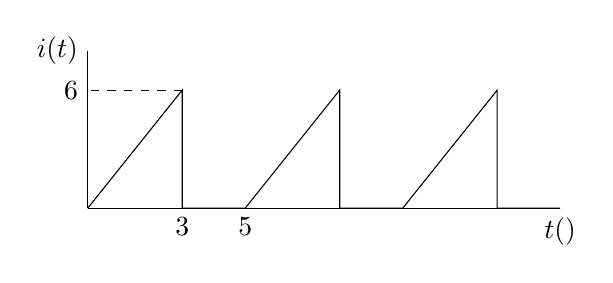
\begin{tikzpicture}
\pgfmathsetmacro{\iP}{1.5};
\pgfmathsetmacro{\T}{2};
\pgfmathsetmacro{\tON}{0.6*\T}
\pgfmathsetmacro{\tOFF}{\T-\tON}
\draw(0,0)--++(6,0)node[below]{$t(\si{\second})$};
\draw(0,0)--(0,2)node[left]{$i(t)$};
\draw(0,0)
\foreach \i in {1,2,3}{--++(\tON,\iP)--++(0,-\iP)--++(\tOFF,0)};
\draw[dashed](\tON,\iP)--++(-\tON,0)node[left]{$\SI{6}{\ampere}$};
\draw(\tON,0) node[below]{$3$};
\draw(\T,0) node[below]{$5$};
\end{tikzpicture}
\caption{مثال \حوالہ{مثال_طاقت_موثر_قیمتیں_پ} کا دور۔}
\label{شکل_طاقت_موثر_قیمتیں_پ}
\end{figure}

حل:یہاں دباو مسلسل تبدیل ہو رہا ہے لہٰذا اس کے خط کی مساوات درکار ہو گی۔دباو کا سیدھا خط \عددی{(0,0)} تا \عددی{(3,6)} خطی تفاعل ہے جس کی شرح ڈھال درج ذیل ہے۔
\begin{align*}
m&=\frac{y_2-y_1}{x_2-x_1}=\frac{6-0}{3-0}=2
\end{align*}
کارتیسی محدد پر \عددی{(0,0)} سے گزرتے \عددی{m} شرح ڈھال کے خط کی مساوات \عددی{y=mx} لکھی جاتی ہے لہٰذا دباو کے خط کی مساوات درج ذیل ہے۔
\begin{align*}
v(t)=2t
\end{align*}
موثر دباو درج ذیل ہے۔
\begin{align*}
v_{\textup{rms}}&=\sqrt{\frac{1}{T} \int_{0}^{T} v^2(t) \dif t}\\
&=\sqrt{\frac{1}{5} \left[\int_{0}^{3} (2t)^2 \dif t+\int_{3}^{5} 0^2 \dif t\right]}\\
&=\sqrt{\left. \left(\frac{1}{5}\right)\left( \frac{4}{3}\right)t^3 \right|_{0}^{3}}\\
&=\SI{2.68}{\volt}
\end{align*} 

\انتہا{مثال}
%==========================

 
%================
\ابتدا{مشق}\شناخت{مشق_طاقت_مشق_موثر_قیمتیں_الف}
شکل \حوالہ{شکل_طاقت_مشق_موثر_قیمتیں_الف} میں دیے دباو کی موثر قیمت دریافت کریں۔
\begin{figure}
\centering
\begin{tikzpicture}
\pgfmathsetmacro{\vP}{2}
\pgfmathsetmacro{\T}{2};
\pgfmathsetmacro{\tON}{0.4*\T}
\pgfmathsetmacro{\tOFF}{\T-\tON}
\draw(0,0)--++(7,0)node[below]{$t(\si{\second})$};
\draw(0,-1)--(0,2.5)node[left]{$v(t)$};
\draw(0,-0.5)
\foreach \i in {1,2,3}{--++(0,\vP)--++(\tON,0)--++(0,-\vP)--++(\tOFF,0)};
\draw(0,1.5)node[left]{$\SI{4}{\volt}$};
\draw[dashed](\tON,-0.5)--++(-\tON,0)node[left]{$\SI{-1}{\volt}$};
\draw(\tON,0) node[below left]{$2$};
\draw(\T,0) node[below right]{$5$};
\end{tikzpicture}
\caption{مشق \حوالہ{مشق_طاقت_مشق_موثر_قیمتیں_الف} کا دور۔}
\label{شکل_طاقت_مشق_موثر_قیمتیں_الف}
\end{figure}

جواب:\عددی{\sqrt{7}\,\si{\volt}}
\انتہا{مشق}
%=======================
\ابتدا{مشق}\شناخت{مشق_طاقت_مشق_موثر_قیمتیں_ب}
شکل \حوالہ{شکل_طاقت_مشق_موثر_قیمتیں_ب} میں \عددی{\SI{3}{\ohm}} مزاحمت کی رو دکھائی گئی ہے۔مزاحمت میں اوسط طاقت کا ضیاع حاصل کریں۔
\begin{figure}
\centering
\begin{tikzpicture}
\pgfmathsetmacro{\iP}{0.5}
\pgfmathsetmacro{\T}{2};
\pgfmathsetmacro{\tON}{0.6*\T}
\pgfmathsetmacro{\tOFF}{\T-\tON}
\draw(0,0)--++(7,0)node[below]{$t(\si{\second})$};
\draw(0,0)--(0,2)node[left]{$i(t)$};
\draw(0,0.5)
\foreach \i in {1,2,3}{--++(\tON,0)--++(0,\iP)--++(\tOFF,0)--++(0,-\iP)};
\draw(0,0.5)node[left]{$\SI{6}{\ampere}$};
\draw[dashed](\tON,1)--++(-\tON,0)node[left]{$\SI{12}{\ampere}$};
\draw(\tON,0) node[below]{$9$};
\draw(\T,0) node[below]{$15$};
\draw(\T+\tON,0) node[below]{$24$};
\draw(2*\T,0) node[below]{$30$};
\end{tikzpicture}
\caption{مشق \حوالہ{مشق_طاقت_مشق_موثر_قیمتیں_ب} کا دور۔}
\label{شکل_طاقت_مشق_موثر_قیمتیں_ب}
\end{figure}

جواب:\عددی{\SI{237.6}{\watt}}
\انتہا{مشق}
%=====================
\ابتدا{مشق}\شناخت{مشق_طاقت_مشق_موثر_قیمتیں_پ}
شکل \حوالہ{شکل_طاقت_مشق_موثر_قیمتیں_پ} میں \عددی{\SI{7}{\ohm}} مزاحمت کی رو دکھائی گئی ہے۔مزاحمت میں اوسط طاقت کا ضیاع دریافت کریں۔
\begin{figure}
\centering
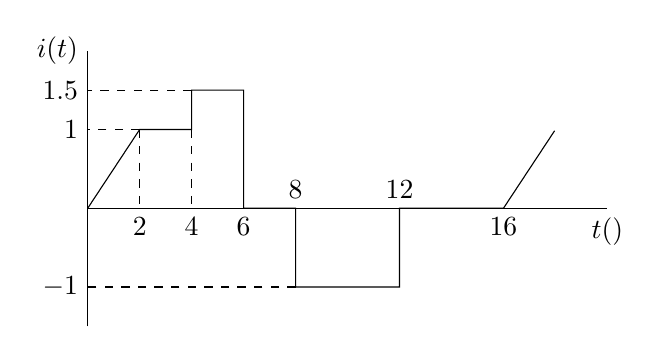
\begin{tikzpicture}[xscale=0.33]
\draw(0,0)--++(20,0)node[below]{$t(\si{\second})$};
\draw(0,-1.5)--(0,2)node[left]{$i(t)$};
\draw(0,0)--(2,1)--(4,1)--(4,1.5)--(6,1.5)--(6,0)--(8,0)--(8,-1)--(12,-1)--(12,0)--(16,0)--++(26.56:2.2);
\draw[dashed](2,1)--++(-2,0)node[left]{$\SI{1}{\ampere}$};
\draw[dashed](4,1.5)--++(-4,0)node[left]{$\SI{1.5}{\ampere}$};
\draw[dashed](8,-1)--++(-8,0)node[left]{$\SI{-1}{\ampere}$};
\draw[dashed](2,1)--++(0,-1)node[below]{$2$};
\draw[dashed](4,1)--++(0,-1)node[below]{$4$};
\draw(6,0)node[below]{$6$};
\draw(8,0)node[above]{$8$};
\draw(12,0)node[above]{$12$};
\draw(16,0)node[below]{$16$};
\end{tikzpicture}
\caption{مشق \حوالہ{مشق_طاقت_مشق_موثر_قیمتیں_پ} کا دور۔}
\label{شکل_طاقت_مشق_موثر_قیمتیں_پ}
\end{figure}

جواب:\عددی{\SI{4.885}{\watt}}
\انتہا{مشق}
%==================

\حصہ{جزو طاقت}
مساوات \حوالہ{مساوات_طاقت_عمومی_پ} اوسط طاقت دیتی ہے۔
\begin{align}
P&=\Vrms \Irms \cos(\theta_v-\theta_i)
\end{align}
اس مساوات میں \عددی{\Vrms\Irms} کے حاصل ضرب کو \اصطلاح{ظاہری طاقت}\فرہنگ{ظاہری طاقت}\فرہنگ{طاقت!ظاہری}\حاشیہب{apparent power}
\فرہنگ{power!apparent} کہا جاتا ہے جبکہ \عددی{P} کو \اصطلاح{حقیقی طاقت}\فرہنگ{حقیقی طاقت}\فرہنگ{طاقت!حقیقی}\حاشیہب{real power}
\فرہنگ{power!real} کہا جاتا ہے۔ظاہری طاقت کو \اصطلاح{وولٹ ایمپیئر}\فرہنگ{وولٹ ایمپیئر}\حاشیہب{volt-ampere}\فرہنگ{volt-ampere} \عددی{\si{\volt\ampere}} میں ناپا جاتا ہے جبکہ حقیقی طاقت کو واٹ \عددی{\si{\watt}} میں ناپا جاتا ہے۔یاد رہے کہ \عددی{\cos(\theta_v-\theta_i)} بے بعد مقدار ہے لہٰذا حقیقی طاقت کا بعد بھی حقیقت میں وولٹ ایمپیئر \عددی{\si{\volt\ampere}} ہی ہے جسے واٹ \عددی{\si{\watt}} کا خصوصی نام دیا گیا ہے۔حقیقی طاقت اور ظاہری طاقت میں فرق ظاہر کرنے اور انہیں پہچانے کی خاطر ان کی اکایوں کو علیحدہ علیحدہ نام دیے گئے ہیں۔

حقیقی طاقت اور ظاہری طاقت کی شرح کو \اصطلاح{جزو طاقت}\فرہنگ{جزو طاقت}\فرہنگ{طاقت!جزو}\حاشیہب{power factor, pf}\فرہنگ{power factor} \عددی{\pf} کہا جاتا ہے۔درج بالا مساوات کی مدد سے جزو طاقت کو درج ذیل لکھا جا سکتا ہے
\begin{align}
\text{\RL{جزو طاقت}}=\pf=\frac{P}{\Vrms\Irms}=\cos(\theta_v-\theta_i)
\end{align}
جہاں 
\begin{align}
\cos(\theta_v-\theta_i)=\cos \theta_{z}
\end{align}
کے برابر ہے۔زاویہ \عددی{\theta_v-\theta_i} درحقیقت بوجھ کے رکاوٹ کا زاویہ ہٹاو \عددی{\theta_{z}} ہے اور اسے \اصطلاح{زاویہ جزو طاقت}\فرہنگ{زاویہ جزو طاقت}\حاشیہب{power factor angle}\فرہنگ{power factor angle} کہا جاتا ہے۔چونکہ \عددی{\cos(\theta_v-\theta_i)=\cos(\theta_i-\theta_v)} کے برابر ہے لہٰذا جزو طاقت کو  امالی بوجھ کی صورت میں \اصطلاح{امالی جزو طاقت}\فرہنگ{جزو طاقت!امالی}\فرہنگ{امالی!جزو طاقت}\حاشیہب{inductive power factor}\فرہنگ{power factor!inductive}
\فرہنگ{inductive!power factor} یا \اصطلاح{پیچھے جزو طاقت}\فرہنگ{جزو طاقت!پیچھے}\حاشیہب{lagging power factor}\فرہنگ{power factor!lagging} کہا جاتا ہے جبکہ برق گیر بوجھ کی صورت میں اس کو \اصطلاح{برق گیر جزو طاقت}\فرہنگ{برق گیر!جزو طاقت}\فرہنگ{جزو طاقت!برق گیر}\حاشیہب{capacitive power factor}\فرہنگ{power factor!capacitive}\فرہنگ{capacitive!power factor} یا \اصطلاح{آگے جزو طاقت}\فرہنگ{آگے جزو طاقت}\فرہنگ{جزو طاقت!آگے}\حاشیہب{leading power factor}\فرہنگ{leading!power factor}\فرہنگ{power factor!leading} کہا جاتا ہے۔اسی طرح امالی بوجھ کی صورت میں زاویہ جزو طاقت کو \اصطلاح{امالی زاویہ جزو طاقت}\فرہنگ{امالی!زاویہ جزو طاقت}\فرہنگ{زاویہ!امالی جزو طاقت} یا \اصطلاح{پیچھے زاویہ جزو طاقت}\فرہنگ{پیچھے زاویہ جزو طاقت}\فرہنگ{پیچھے!زاویہ جزو طاقت}\فرہنگ{زاویہ!پیچھے جزو طاقت} کہا جاتا ہے جبکہ برق گیر بوجھ کی صورت میں اس کو  \اصطلاح{برق گیر زاویہ جزو طاقت}\فرہنگ{برق گیر زاویہ جزو طاقت}\فرہنگ{زاویہ!برق گیر جزو طاقت} یا \اصطلاح{آگے زاویہ جزو طاقت}\فرہنگ{آگے زاویہ جزو طاقت}\فرہنگ{زاویہ!آگے جزو طاقت} کہا جاتا ہے۔ 

مزاحمتی بوجھ کا \عددی{\theta_z=0^{\circ}} ہوتا ہے لہٰذا مزاحمتی بوجھ کا جزو طاقت \عددی{\cos \theta_z=1} ہو گا۔  امالہ گیر کا \عددی{\theta_z=90^{\circ}} ہے لہٰذا اس کا \عددی{\cos \theta_z=0} ہے۔برق گیر کا \عددی{\theta_z=-90^{\circ}} ہے لہٰذا اس کا \عددی{\cos \theta_z=0} ہے۔مزاحمت اور امالہ گیر پر مبنی دور کے رکاوٹ کا زاویہ \عددی{0^{\circ}} تا \عددی{90^{\circ}} ممکن ہے لہٰذا ایسے دور کا امالی جزو طاقت \عددی{1} تا \عددی{0} ممکن ہے۔اسی طرح برق گیر اور مزاحمت پر مبنی دور کے رکاوٹ کا زاویہ \عددی{0^{\circ}} تا \عددی{-90^{\circ}} ممکن ہے لہٰذا ایسے دور کا برق گیر جزو طاقت  \عددی{1} تا \عددی{0} ممکن ہے۔مزاحمت، امالہ اور برق گیر پر مبنی دور کے رکاوٹ کا زاویہ \عددی{-90^{\circ}} سے \عددی{0^{\circ}} تا \عددی{^{\circ}90} ممکن ہے لہٰذا ایسے دور کا جزو طاقت تینوں اقسام کا ممکن ہے۔

آگے زاویہ اور پیچھے زاویہ سے مراد دباو کے لہٰذا سے رو کا زاویہ ہے۔چونکہ امالی دور میں دباو سے رو پیچھے رہتی ہے لہٰذا ایسے ادوار \اصطلاح{پیچھے ادوار} کہلاتے ہیں اور ان کا زاویہ اور جزو طاقت بھی \اصطلاح{پیچھے} کہلاتے ہیں۔اس کے برعکس برق گیر دور میں دباو سے رو آگے رہتی ہے لہٰذا ان ادوار کو \اصطلاح{آگے ادوار} کہتے ہیں اور ان کا زاویہ اور جزو طاقت بھی \اصطلاح{آگے} کہلاتے ہیں۔یوں امالی بوجھ \عددی{Z_L=2+j6} کا زاویہ \عددی{\tan^{-1}\tfrac{6}{2}=71.57^{\circ}}  اور پیچھے جزو طاقت \عددی{\cos 71.57^{\circ}=0.316} ہے۔اسی طرح برق گیر بوجھ \عددی{Z_C=3-j4} کا زاویہ \عددی{\tan^{-1} \left(-\tfrac{4}{3}\right)=-53.13^{\circ}} اور آگے جزو طاقت \عددی{\cos(-53.13^{\circ})=0.6} ہے۔
%=============================
\ابتدا{مثال}\شناخت{مثال_طاقت_جزو_طاقت_کی_اہمیت}
ایک صنعت کو \عددی{560 \, \si{\volt} \, \rms} پر \عددی{\SI{100}{\kilo\watt}} طاقت مہیا کیا جاتا ہے۔صنعتی بوجھ کا جزو طاقت \عددی{0.68} امالی ہے۔برقی طاقت کو منبع سے بوجھ تک \اصطلاح{ترسیلی تاروں}\فرہنگ{ترسیلی تار}\حاشیہب{transmission lines}\فرہنگ{transmission lines}\حاشیہد{پاکستان میں بجلی کے کھمبوں پر ترسیلی تار آپ نے ضرور دیکھے ہوں گے۔ڈیم میں موجود بجلی گھر سے صارف تک طاقت انہیں ترسیلی تاروں کے ذریعہ پہنچتا ہے۔} کے ذریعہ پہنچایا جاتا ہے۔ترسیلی تار کی مزاحمت \عددی{\SI{0.06}{\ohm}} ہے۔ترسیلی تار میں طاقت کا ضیاع دریافت کریں۔منبع طاقت کتنا طاقت پیدا کرے گا۔اگر صنعتی بوجھ کا جزو طاقت \عددی{0.95} امالی کر دیا جائے تب جوابات کیا ہوں گے۔
\begin{figure}
\centering
\begin{tikzpicture}[american voltages]
\draw(0,0) to [american voltage source,l={$\hat{V}_{\textup{m}}$}]++(0,\y) to [resistor,i={$\bIrms$},l={$\SI{0.06}{\ohm}$}]++(2*\x,0) to [european resistor,v={$\SI{560}{\volt}\,\rms$},l={$\substack{\displaystyle \SI{100}{\kilo\watt} \\ \displaystyle 0.68 \, \text{امالی}}$}]++(0,-\y) to [short] (0,0);
\end{tikzpicture}
\caption{اکائی جزو طاقت بہترین ہے۔}
\label{شکل_طاقت_جزو_طاقت_کے_اثرات}
\end{figure}

حل:شکل \حوالہ{شکل_طاقت_جزو_طاقت_کے_اثرات} میں صورت حال دکھائی گئی ہے۔مساوات \حوالہ{مساوات_طاقت_عمومی_پ} سے رو حاصل کرتے ہیں جہاں \عددی{\cos(\theta_v-\theta_i)} جزو طاقت ہے۔
\begin{align*}
\Irms&=\frac{P}{\Vrms \cos(\theta_v-\theta_i)}\\
&=\frac{\num{100000}}{(560)(0.68)}\\
&=\SI{263}{\ampere}\,\rms
\end{align*}
تار کی مزاحمت میں ضائع ہونے والے طاقت کا حساب کرتے ہیں۔
\begin{align*}
P_{\text{تار}}&=(263^2)(0.06)=\SI{4.138}{\watt}
\end{align*}
یوں منبع کو درج ذیل طاقت فراہم کرنا ہو گا
\begin{align*}
P_{\text{منبع}}=\SI{100}{\kilo\watt}+\SI{4.138}{\kilo\watt}=\SI{104.138}{\kilo\watt}
\end{align*} 
جس میں سے \عددی{\SI{4.138}{\kilo\watt}} مسلسل ضائع ہو رہا ہے۔

اس کے برعکس \عددی{0.95} امالی جزو طاقت کی صورت میں درج ذیل ہو گا۔
\begin{align*}
\Irms&=\frac{\num{100000}}{(560)(0.95)}=\SI{188}{\ampere}\\
P_{\text{تار}}&=(188^2)(0.06)=\SI{2.12}{\watt}\\
P_{\text{منبع}}&=\SI{100}{\kilo\watt}+\SI{2.12}{\watt}=\SI{102.12}{\kilo\watt}
\end{align*}
آپ دیکھ سکتے ہیں کہ صرف جزو طاقت تبدیل کرنے سے طاقت کا ضیاع \عددی{\SI{4.138}{\kilo\watt}} سے کم ہو کر \عددی{\SI{2.12}{\kilo\watt}} ہو گیا ہے۔
\انتہا{مثال}
%============================

آپ نے مثال \حوالہ{مثال_طاقت_جزو_طاقت_کی_اہمیت} میں دیکھا کہ جزو طاقت کی تبدیلی سے ترسیلی تاروں میں طاقت کے ضیاع تبدیل ہوتا ہے۔مساوات \حوالہ{مساوات_طاقت_عمومی_پ} سے ظاہر ہے کہ جزو طاقت کی قیمت بڑھانے سے رو کی قیمت کم ہوتی ہے۔جزو طاقت کی زیادہ سے زیادہ قیمت اکائی ہے۔یوں اکائی جزو طاقت پر کم سے کم رو درکار ہو گی۔کم سے کم ور کی صورت میں ترسیلی تاروں میں طاقت کا ضیاع کم سے کم ہو گا۔ی

ہاں رک کر تسلی کر لیں کہ مثال \حوالہ{مثال_طاقت_جزو_طاقت_کی_اہمیت} میں \عددی{0.68} آگے جزو طاقت پر بھی \عددی{\Irms=\SI{263}{\ampere}} ہو گا لہٰذا  مسائل اتنے ہی بُرے ہوں گے جتنے \عددی{0.68} پیچھے جزو طاقت پر ہیں۔

بجلی کا میٹر صارف کے ہاں نسب ہوتا ہے جو خرچ کیے توانائی کا حساب رکھتا ہے۔یہ میٹر ترسیلی تاروں میں ضائع توانائی کو نہیں ناپ سکتا۔برقی طاقت کے پیدا کار صنعت کو صارف کی درکار طاقت کے ساتھ ساتھ ترسیلی تاروں میں ضائع ہونے والا طاقت بھی پیدا کرنا پڑتا ہے لہٰذا ان کی دلچسپی اس بات میں ہو گی کہ ترسیلی تاروں میں طاقت کا ضیاع کم سے کم ہو۔یہی وجہ ہے کہ پیدا کار صنعت کوشش کرتی ہے کہ صارف کو مجبور کرے کہ اس کا جزو طاقت اکائی کے قریب ترین ہو۔اگر صارف اپنے جزو طاقت پر قابو نہیں پاتا تو پیدا کار اس پر جرمانہ عائد کرتا ہے۔اس کتاب کے لکھتے وقت پاکستان میں \عددی{0.9} سے کم جزو طاقت کی صورت میں صارف صنعت پر جرمانہ عائد کیا جاتا ہے البتہ گھریلو صارفین پر فی الحال کم جزو طاقت کی صورت میں کوئی جرمانہ عائد نہیں کیا جاتا۔عموماً صنعتوں میں بوجھ کا بیشتر حصہ مختلف اقسام کے موٹر پر مبنی ہوتا ہے جو امالی بوجھ ہے۔یہی وجہ ہے کہ جب بھی صنعتی بوجھ کی بات کی جائے تو امالی بوجھ کی بات کی جاتی ہے۔  

حصہ \حوالہ{حصہ_طاقت_جزو_طاقت_پر_قابو} میں جزو طاقت پر قابو پانے پر غور کیا جائے گا۔
%============================
\ابتدا{مشق}
ایک صنعت کو \عددی{\SI{50}{\hertz}} تعدد اور \عددی{\SI{480}{\volt}\,\rms} دباو پر \عددی{\SI{60}{\kilo\watt}} طاقت \عددی{\SI{0.2}{\ohm}} مزاحمت کے ترسیلی تاروں کے ذریعہ فراہم کیا جاتا ہے۔ صارف اپنا جزو طاقت \عددی{0.64} امالی سے بہتر کرتے ہوئے \عددی{0.98} امالی کر دیتا ہے۔طاقت میں بچت دریافت کریں۔   

جواب:\عددی{\SI{4.376}{\kilo\watt}}
\انتہا{مشق}
%===========================
\حصہ{مخلوط طاقت}
برقرار حال بدلتی رو طاقت پر غور کرنے کے لئے \اصطلاح{مخلوط طاقت}\فرہنگ{مخلوط طاقت}\فرہنگ{طاقت!مخلوط}\حاشیہب{complex power}\فرہنگ{complex power}\فرہنگ{power!complex} کا جاننا ضروری ہے لہٰذا اس حصے میں مخلوط طاقت پر بحث کی جائے گی۔   
\begin{figure}
\centering
\begin{tikzpicture}
\draw (0,0)--++(0.5,0)--++(0,2.5)--++(-0.5,0)--++(0,-2.5);
\draw(0.25,1.25)node[rotate=90]{\RL{بدلتی رو دور}};
\draw(0.5,2.25) to [short,i={$\bIrms$}]++(\x,0) to [european resistor,l={$\bZ$}]++(0,-\y) to [short] ++(-\x,0);
\draw(0.5+\x/2,1.25)node{$\begin{aligned}&+ \\& \bVrms \\ &-\end{aligned}$};
\end{tikzpicture}
\caption{طاقت کے اقسام پر غور کے لئے دور۔}
\label{شکل_طاقت_اقسام_طاقت}
\end{figure}

شکل \حوالہ{شکل_طاقت_اقسام_طاقت} میں عمومی دور دکھایا گیا ہے جہاں درج ذیل ہیں۔
\begin{align*}
\bVrms&=\Vrms\phase{\theta_v}=V_{\text{حقیقی}}+j V_{\text{خیالی}}\\
\bIrms&=\Irms\phase{\theta_i}=I_{\text{حقیقی}}+j I_{\text{خیالی}}\\
\bZ&=Z\phase{\theta_z}=R+jX
\end{align*}
رو \عددی{\bIrmsCC} سے مراد \عددی{\bIrms} کا جوڑی دار مخلوط ہے۔
\begin{align*}
\bIrmsCC&=\Irms\phase{-\theta_i}=I_{\text{حقیقی}}-j I_{\text{خیالی}}
\end{align*}
مخلوط طاقت \عددی{\bS} کی تعریف
\begin{align}\label{مساوات_طاقت_مخلوط_طاقت_الف}
\bS=\bVrms\bIrmsCC
\end{align}
ہے جس میں دباو اور رو کی قیمتیں پر کرتے ہوئے 
\begin{gather}
\begin{aligned}\label{مساوات_طاقت_مخلوط_طاقت_ب}
\bS&=\Vrms \phase{\theta_v}\Irms\phase{-\theta_i}\\
&=\Vrms \Irms \phase{\theta_v-\theta_i}\\
&=\Vrms\Irms \cos(\theta_v-\theta_i)+j\Vrms\Irms \sin(\theta_v-\theta_i)
\end{aligned}
\end{gather}
ملتا ہے جہاں \عددی{\theta_v-\theta_i=\theta_z} کے برابر ہے۔مساوات \حوالہ{مساوات_طاقت_مخلوط_طاقت_ب} کا حقیقی جزو درحقیقت حقیقی اوسط طاقت \عددی{P} ہے جبکہ اس کے خیالی جزو \عددی{Q} کو \اصطلاح{متعاملی طاقت}\فرہنگ{متعاملی طاقت}\فرہنگ{طاقت!متعاملی}\حاشیہب{reactive power}\فرہنگ{power!reactive}\فرہنگ{reactive!power} یا \اصطلاح{تربیعی طاقت}\فرہنگ{طاقت!تربیعی}\فرہنگ{تربیعی!طاقت}\حاشیہب{quadrature power}\فرہنگ{power!quadrature} کہا جاتا ہے۔یوں مخلوط طاقت کو درج ذیل لکھا جا سکتا ہے
\begin{align}\label{مساوات_طاقت_مخلوط_طاقت_مساوی_حقیقی_متعاملی}
\bS=P+jQ
\end{align}
جہاں
\begin{align}
P&=\left. \bS \right|_{\text{حقیقی}}=\Vrms \Irms \cos(\theta_v-\theta_i) \label{مساوات_طاقت_مخلوط_طاقت_پ}\\
Q&=\left. \bS \right|_{\text{خیالی}}=\Vrms \Irms \sin(\theta_v-\theta_i)\label{مساوات_طاقت_مخلوط_طاقت_ت}
\end{align}
ہیں۔مساوات \حوالہ{مساوات_طاقت_مخلوط_طاقت_ب} سے ظاہر ہے کہ مخلوط طاقت کے حیطے  کو ہم ظاہری طاقت کہتے ہیں جبکہ مخلوط طاقت کے زاویہ کو ہم زاویہ جزو طاقت کہتے ہیں۔ مخلوط طاقت کو ظاہری طاقت کی طرح وولٹ ایمپیئر \عددی{\si{\volt\ampere}} میں ناپا جاتا ہے، حقیقی طاقت کو واٹ \عددی{\si{\watt}} میں ناپا جاتا ہے جبکہ متعاملی طاقت \عددی{Q} کو، شناخت کی خاطر، متعاملی وولٹ ایمپیئر \عددی{\si{\var}} میں ناپا جاتا ہے۔یاد رہے کہ ان تمام اقسام کے طاقتوں کا بعد وولٹ ایمپیئر \عددی{\si{\volt\ampere}} ہی ہے۔
%==================
\ابتدا{مثال}
رو  \عددی{\bIrms=I_h+jI_k} کی مقدار \عددی{\Irms} حاصل کریں۔رو \عددی{\bIrmsCC=I_h-jI_k} کی مقدار بھی حاصل کریں۔ان رو کا حاصل ضرب دریافت کریں۔

حل:دی گئی رو کی مقداریں درج ذیل ہیں۔
\begin{align*}
\abs{\bIrms}&=\sqrt{I_h^2+I_k^2}=\Irms\\
\abs{\bIrmsCC}&=\sqrt{I_h^2+(-I_k)^2}=\Irms
\end{align*}
دونوں  کا حاصل ضرب درج ذیل ہے۔
\begin{align}\label{مساوات_طاقت_مقدار_مساوی_مخلوط_اور_جوڑی_دور_ضرب}
\bIrms\bIrmsCC&=(I_h+jI_k)(I_h-jI_k)=I_h^2+I_k^2=\IrmsS
\end{align}
\انتہا{مثال}
%====================
آئیں مساوات \حوالہ{مساوات_طاقت_مخلوط_طاقت_پ} اور مساوات \حوالہ{مساوات_طاقت_مخلوط_طاقت_ت} پر مزاحمت، امالہ اور برق گیر کے نقطہ نظر سے مزید غور کریں۔مزاحمت کا \عددی{\theta_v-\theta_i=0^{\circ}} ہے لہٰذا اس کے \عددی{\cos(\theta_v-\theta_i)=1} اور \عددی{\sin(\theta_v-\theta_i)=0} ہیں۔یوں مزاحمت حقیقی طاقت جذب \عددی{(P>0)} کرتا ہے جبکہ یہ متعاملی طاقت کو جذب نہیں کرتا لہٰذا \عددی{Q=0} ہے۔امالہ کا \عددی{\theta_v-\theta_i=90^{\circ}}  لہٰذا
\begin{align}
P&=\Vrms \Irms \cos 90^{\circ}=0\\
Q&=\Vrms \Irms \sin 90^{\circ}>0
\end{align}
ہیں۔امالہ گیر متعاملی طاقت کو جذب کرتا ہے جبکہ یہ حقیقی طاقت کو جذب نہیں کرتا۔برق گیر کا \عددی{\theta_v-\theta_i=-90^{\circ}} لہٰذا
\begin{align}
P&=\Vrms \Irms \cos (-90^{\circ})=0\\
Q&=\Vrms \Irms \sin (-90^{\circ})<0
\end{align}
ہیں۔برق گیر حقیقی طاقت جذب نہیں کرتا جبکہ یہ متعاملی طاقت مہیا کرتا ہے۔

ہم نے دیکھا کہ مزاحمت حقیقی طاقت جذب کرتا ہے جبکہ امالہ گیر اور برق گیر بالترتیب متعاملی طاقت جذب اور مہیا کرتے ہیں۔ ان پرزوں میں بنیادی فرق یہ ہے کہ مزاحمت میں طاقت ضائع ہوتا ہے جبکہ امالہ گیر اور برق گیر طاقت ذخیرہ کرتے ہوئے اسے دور کو واپس منتقل کرنے کی صلاحیت رکھتے ہیں۔ان حقائق سے ہم کہہ سکتے ہیں کہ متعاملی طاقت کا تعلق طاقت ذخیرہ کرنے سے  ہے۔  

آئیں مساوات \حوالہ{مساوات_طاقت_مخلوط_طاقت_الف} میں \عددی{\bVrms=\bIrms \bZ} پر کریں
\begin{align}
\bS=\bVrms\bIrmsCC=\bIrms\bZ\bIrmsCC=\IrmsS\bZ=\IrmsS(R+jX)=P+jQ
\end{align}
جہاں مساوات \حوالہ{مساوات_طاقت_مقدار_مساوی_مخلوط_اور_جوڑی_دور_ضرب} اور مساوات \حوالہ{مساوات_طاقت_مخلوط_طاقت_مساوی_حقیقی_متعاملی} کا سہارا لیا گیا ہے۔اسی طرح مساوات \حوالہ{مساوات_طاقت_مخلوط_طاقت_الف} میں دباو کی بجائے رو کے لئے پر کرتے ہوئے درج ذیل لکھا جا سکتا ہے۔
\begin{align}
\bS=\bVrms\left(\frac{\bVrms}{\bZ}\right)^*=\frac{\VrmsS}{\bZCC}=\VrmsS \bYCC=\VrmsS(B+jG)^*=P+jQ
\end{align}
اس مساوات کے تحت جوڑی دار مخلوط فراوانی کو دباو کی موثر قیمت سے ضرب دیتے ہوئے فراوانی کی طاقت حاصل کی جا سکتی ہے۔یہ وہ طاقت ہے جو فراوانی جذب کرتا ہے۔  یوں اگر شکل \حوالہ{شکل_طاقت_اقسام_طاقت} میں برق گیر بطور بوجھ \عددی{\bZ} نسب ہوتا تب فراوانی \عددی{j\omega C} کے برابر ہوتی جسے درج بالا مساوات میں پر کرتے ہوئے
\begin{align}\label{مساوات_طاقت_برق_گیر_مخلوط_طاقت}
\bS=\VrmsS (j\omega C)^*=-j\omega C \VrmsS
\end{align}
ملتا ہے۔آپ نے دیکھا کہ مخلوط طاقت کی قیمت منفی ہے۔یوں برق گیر متعاملی طاقت فراہم کرتا ہے۔

شکل \حوالہ{شکل_طاقت_طاقتی_تعلقات} طاقت کے تعلقات پر  مزید روشنی ڈالتا ہے۔شکل-الف کے تحت رو کو دو ٹکڑوں میں تقسیم کیا جا سکتا ہے۔پہلا ٹکڑا \عددی{\bVrms} کے ہم زاویہ ہے جبکہ دوسرا ٹکڑا دباو کے ساتھ \عددی{90^{\circ}} کا زاویہ بناتا ہے۔مساوات \حوالہ{مساوات_طاقت_مخلوط_طاقت_پ} کے تحت دباو اور اس کے ہم زاویہ رو مل کر حقیقی طاقت \عددی{P} پیدا کرتے ہیں۔اسی طرح مساوات \حوالہ{مساوات_طاقت_مخلوط_طاقت_ت} کے تحت دباو اور دباو کے عمودی رو مل کر متعاملی طاقت \عددی{Q} پیدا کرتے ہیں۔انہیں دو مساوات سے درج ذیل تعلق بھی حاصل ہوتا ہے
\begin{align}
\tan(\theta_v-\theta_i)=\frac{Q}{P}
\end{align}
جس کو شکل-ب کے \اصطلاح{طاقتی تکون}\فرہنگ{طاقتی تکون}\فرہنگ{تکون!طاقت}\حاشیہب{power triangle}\فرہنگ{power triangle} سے بھی حاصل کیا جا سکتا ہے۔
 شکل-ب امالی بوجھ کے لئے دکھایا گیا ہے جہاں \عددی{\theta_v-\theta_i>0} ہے۔چونکہ زاویہ افقی محور سے گھڑی کی گردش کے الٹ جانب گھومتے ہوئے ناپا جاتا ہے لہٰذا مثبت زاویہ حقیقی محور سے اوپر کو ہو گا۔یوں امالی بوجھ کا \عددی{Q} مثبت ہے۔برق گیر بوجھ کی صورت میں \عددی{\theta_v-\theta_i<0} ہو گا لہٰذا \عددی{\bS} کا خط حقیقی محور سے نیچے کو ہو گا لہٰذا \عددی{Q} کی قیمت منفی ہو گی۔مزاحمتی بوجھ کی صورت میں \عددی{\theta_v-\theta_i=0} ہو گا لہٰذا \عددی{\bS} کا خط عین حقیقی محور پر ہو گا لہٰذا مخلوط طاقت اور حقیقی طاقت برابر ہوں گے جبکہ متعاملی طاقت صفر ہو گا۔

آخر میں بتلاتا چلوں کہ دور میں حقیقی طاقت کی طرح مخلوط طاقت پر بھی بقائے توانائی کا قانون لاگو ہوتا ہے۔

\begin{figure}
\centering
\begin{subfigure}{0.5\textwidth}
\centering
\begin{tikzpicture}
\pgfmathsetmacro{\lenV}{4}
\pgfmathsetmacro{\lenI}{3.5}
\pgfmathsetmacro{\angV}{40}
\pgfmathsetmacro{\angI}{20}
\draw(0,0)--++(4,0)node[below]{\text{حقیقی}};
\draw(0,0)--++(0,2.5)node[left]{\text{خیالی}};
\draw[-latex](0,0)coordinate(O)--++(\angV:\lenV)node[above]{$\bVrms$}coordinate(vTip);
\draw[-latex](0,0)--++(\angI:\lenI)node[below]{$\bIrms$}coordinate(iTip);
\draw[latex-](iTip)--($(vTip)!(iTip)!(O)$)coordinate(iDrop)node[pos=0.5,right]{$\bIrms \sin(\theta_v-\theta_i)$};
\draw[-latex](O)--(iDrop)node[pos=0.55,above,sloped]{$\bIrms \cos(\theta_v-\theta_i)$};
\draw[-stealth] ([shift={(0:1)}]0,0) arc (0:\angV:1);
\draw(3/4*\angV:1.3)node[]{$\theta_v$};
\draw[-stealth] ([shift={(0:1.3)}]0,0) arc (0:\angI:1.3);
\draw(1/2*\angI:1.6)node[]{$\theta_i$};
\end{tikzpicture}
\caption*{(الف)}
\end{subfigure}%
\begin{subfigure}{0.5\textwidth}
\centering
\begin{tikzpicture}
\pgfmathsetmacro{\lenS}{3.5}
\pgfmathsetmacro{\angS}{30}
\draw(0,0)--++(4,0)node[below]{\text{حقیقی}};
\draw(0,0)--++(0,2.5)node[left]{\text{خیالی}};
\draw[-latex](0,0)coordinate(O)--++(\angS:\lenS)node[pos=0.7,above]{$\bS$}coordinate(Tip);
\draw[-stealth] ([shift={(0:1.3)}]0,0) arc (0:\angS:1.3);
\draw(1/2*\angS:1.3)node[right]{$\theta_v-\theta_i$};
\draw[latex-](Tip)--($(0,0)!(Tip)!(4,0)$)coordinate(Bot)node[pos=0.5,right]{$Q$};
\draw[-latex](O)--(Bot)node[pos=0.7,below]{$P$};
\end{tikzpicture}
\caption*{(ب)}
\end{subfigure}%
\caption{طاقتی تعلق۔}
\label{شکل_طاقت_طاقتی_تعلقات}
\end{figure}
%================
\ابتدا{مثال}\شناخت{مثال_طاقت_جزو_طاقت_الف}
امالی بوجھ کو \عددی{\SI{50}{\kilo\watt}} طاقت فراہم کی جا رہی ہے۔بوجھ پر موثر دباو \عددی{\SI{230}{\volt}}، تعدد \عددی{\SI{50}{\hertz}} اور پیچھے جزو طاقت \عددی{0.9} ہے۔ترسیلی تاروں  کی رکاوٹ \عددی{\bZ_{\text{تار}}=0.05+j0.25\,\si{\ohm}} ہے۔ منبع طاقت پر دباو، جزو طاقت اور طاقت کا تخمینہ لگائیں۔
\begin{figure}
\centering
\begin{tikzpicture}[american voltages]
\draw(0,0) to [american voltage source,l={$\hat{V}_{\textup{rms}}$}]++(0,\yy) to [resistor,l={$\SI{0.05}{\ohm}$}]++(\xx,0) to [inductor,l={$j0.25\,\si{\ohm}$}]++(\x,0) to [european resistor,i>^={$\hat{I}_{\textup{rms}}$},v={$230\phase{0^{\circ}}\, \si{\volt\,rms}$},l={$\substack{\displaystyle \SI{50}{\kilo\watt} \\ \displaystyle \text{\RL{پیچھے جزو طاقت \, $0.9$}}}$}]++(0,-\yy) to [short] (0,0);
\end{tikzpicture}
\caption{مثال \حوالہ{مثال_طاقت_جزو_طاقت_الف} کا دور۔}
\label{شکل_طاقت_جزو_طاقت_الف}
\end{figure}

حل:دور کو شکل \حوالہ{شکل_طاقت_جزو_طاقت_الف} میں دکھایا گیا ہے جہاں ترسیلی تار کی رکاوٹ صرف بالائی تار پر دکھائی گئی ہے۔حقیقت میں بالائی اور نچلی تار کی رکاوٹیں سلسلہ وار جڑی ہیں۔ان کا مجموعہ کل رکاوٹ ہے جسے عموماً ایک تار پر دکھایا جاتا ہے۔

بوجھ کے دباو کو حوالہ دوری سمتیہ لیتے ہوئے اس کا زاویہ صفر چننا گیا ہے۔مخلوط طاقت
\begin{align*}
S=\frac{P}{\pf}=\frac{\num{50000}}{0.9}=\num{55556}\,\si{\volt\ampere}
\end{align*}
ہے جبکہ بوجھ پر \عددی{\theta_v-\theta_i=\cos^{-1}(0.9)=25.84^{\circ}} ہے لہٰذا بوجھ پر
\begin{align*}
\bS_L=\num{55556}\phase{25.84^{\circ}}=\num{50000}+j\num{24216} \,\si{\volt\ampere}
\end{align*}
ہو گا۔چونکہ \عددی{\bS_L=\hat{V}_{\textup{rms}}\hat{I}^*_{\textup{rms}}}  ہو لہٰذا
\begin{align*}
\hat{I}_{L,\textup{rms}}=\left(\frac{\num{55556}\phase{25.84^{\circ}}}{230\phase{0^{\circ}}}\right)^*=241.55\phase{-25.84^{\circ}} \, \si{\ampere}\, \textup{rms}
\end{align*}
تار میں مخلوط طاقت کا ضیاع 
\begin{align*}
\bS_{\text{تار}} =I^2_{L,\textup{rms}} \bZ_{\text{تار}}=241.55^2 (0.05+j0.25)=\num{2917}+j\num{14586}\,\si{\volt\ampere}
\end{align*}
ہے۔بقائے توانائی کے تحت یوں منبع طاقت پر مخلوط طاقت درج ذیل ہو گا۔
\begin{align*}
\bS_{\text{منبع}}&=\bS_L+\bS_{\text{تار}}\\
&=\num{50000}+j\num{24216}+\num{2917}+j\num{14586}\\
&=\num{52917}+j\num{38802} \\
&=\num{65619}\phase{36.25^{\circ}}\, \si{\volt\ampere}
\end{align*}
اس طرح منبع کا دباو
\begin{align*}
V_{\textup{rms}}=\frac{\abs{\bS_{\text{منبع}}}}{I_{L,\textup{rms}}}=\frac{\num{65619}}{241.55}=\SI{272}{\volt}
\end{align*}
اور  منبع پر پیچھے جزو طاقت درج ذیل ہو گا۔
\begin{align*}
\pf=\cos 36.25^{\circ}=0.806
\end{align*}

آئیں اسی کو دوبارہ کرخوف مساوات سے حل کریں۔پیچھے جزو طاقت \عددی{0.9} سے رو کا زاویہ حاصل کرتے ہیں جہاں امالی بوجھ کی وجہ سے زاویہ منفی ہو گا۔
\begin{align*}
\theta_i=\cos^{-1} 0.9=-25.84^{\circ}
\end{align*}
بوجھ کی رو حاصل کرتے ہیں۔
\begin{align*}
\Irms=\frac{P}{\Vrms \cos \theta_i}=\frac{\num{50000}}{(230)(0.9)}=\SI{241.55}{\ampere}
\end{align*}
یوں \عددی{\hat{I}_{\textup{rms}}=241.55\phase{-25.84^{\circ}}} ہو گا۔شکل کو دیکھتے ہوئے کرخوف کی مساوات سے درج ذیل لکھا جا سکتا ہے۔
\begin{align*}
\hat{V}_{\textup{rms}}&=230\phase{0^{\circ}}+(241.55\phase{-25.84^{\circ}})(0.05+j0.25)\\
&=272\phase{10.41^{\circ}}\,\si{\volt}
\end{align*}
یوں منبع طاقت پر دباو سے رو
\begin{align*}
10.41^{\circ}-(-25.84^{\circ})=36.25^{\circ}
\end{align*}
پیچھے ہے لہٰذا منبع پر پیچھے جزو طاقت \عددی{\cos(36.25^{\circ})=0.806} ہو گا۔
\انتہا{مثال}
%================
\ابتدا{مثال}
گزشتہ مثال کے شکل \حوالہ{شکل_طاقت_جزو_طاقت_الف} میں بقایا تمام معلومات وہی ہیں البتہ بوجھ پر جزو طاقت پیچھے کی بجائے آگے ہے۔منبع طاقت کا دباو حاصل کریں۔

حل:گزشتہ مثال میں عین ہمارے توقع کے مطابق منبع طاقت کا دباو، بوجھ کے دباو سے زیادہ تھا۔یک سمتی ادوار میں ہم یہی توقع کرتے ہیں کہ زیادہ دباو کے نقطے سے طاقت  کم دباو کے نقطے  کو فراہم ہوتا ہے۔اس مثال میں ہم دیکھیں گے کہ کبھی کبھار ہمارے توقعات غلط ثابت ہوتی ہیں۔ 
 
اس مسئلے کو کرخوف مساوات سے حل کرتے ہیں۔آگے جزو طاقت \عددی{0.9} سے رو کا زاویہ حاصل کرتے ہیں۔آگے جزو طاقت برق گیر بوجھ کی نشاندہی کرتا ہے لہٰذا بوجھ کے رکاوٹ کا زاویہ مثبت ہو گا۔
\begin{align*}
\theta_i=\cos^{-1} 0.9=25.84^{\circ}
\end{align*}
بوجھ کی رو حاصل کرتے ہیں۔
\begin{align*}
\Irms=\frac{P}{\Vrms \cos \theta_i}=\frac{\num{50000}}{(230)(0.9)}=\SI{241.55}{\ampere}
\end{align*}
یوں \عددی{\hat{I}_{\textup{rms}}=241.55\phase{25.84^{\circ}}} ہو گا۔شکل کو دیکھتے ہوئے کرخوف کی مساوات سے درج ذیل لکھا جا سکتا ہے۔
\begin{align*}
\hat{V}_{\textup{rms}}&=230\phase{0^{\circ}}+(241.55\phase{25.84^{\circ}})(0.05+j0.25)\\
&=223\phase{15.53^{\circ}}\,\si{\volt}
\end{align*}
یوں منبع طاقت پر دباو سے رو
\begin{align*}
(25.84^{\circ})-15.53^{\circ}=10.31^{\circ}
\end{align*}
آگے  ہے لہٰذا منبع پر آگے جزو طاقت \عددی{\cos(-10.31^{\circ})=0.98} ہو گا۔آپ دیکھ سکتے ہیں کہ بوجھ پر موثر دباو \عددی{\SI{230}{\volt}} ہے جبکہ منبع طاقت کا موثر دباو \عددی{\SI{223}{\volt}} ہے جو کہ بوجھ کے دباو سے کم ہے۔
\انتہا{مثال}
%===================
\ابتدا{مشق}
شکل \حوالہ{شکل_طاقت_جزو_طاقت_الف} میں بقایا تمام معلومات وہی ہیں البتہ آگے جزو طاقت \عددی{0.8} ہے۔منبع طاقت کا موثر دباو اور جزو طاقت حاصل کریں۔منبع کتنا طاقت پیدا کر رہا ہے۔

جوابات:\عددی{\SI{210}{\volt}\, \textup{rms}}، \عددی{\pf=0.94 \,\text{آگے}}، \عددی{\SI{53.69}{\kilo\watt}}
\انتہا{مشق}
%=================
\ابتدا{مشق}
ایک صنعتی بوجھ کو \عددی{\SI{30}{\kilo\watt}} طاقت \عددی{0.82} پیچھے جزو طاقت پر درکار ہے۔بوجھ پر موثر دباو \عددی{\SI{230}{\volt}} اور تعدد \عددی{\SI{50}{\hertz}} ہے۔منبع سے صنعت تک طاقت کو ترسیلی تاروں کے ذریعہ پہنچایا جاتا ہے۔ان ترسیلی تاروں کی رکاوٹ \عددی{\bZ_{\text{تار}}=0.08+j0.3\,\si{\ohm}} ہے۔ترسیلی تاروں میں حقیقی اور متعاملی طاقت کا ضیاع دریافت کریں۔ترسیلی تار کے داخلی سر پر درکار حقیقی اور متعاملی طاقت دریافت کریں۔

جوابات:\عددی{P_{\text{تار}}=\SI{2024}{\watt}}، \عددی{Q_{\text{تار}}=\SI{7590}{\var}}، \عددی{P_{\text{منبع}}=\SI{32}{\kilo\watt}}، \عددی{Q_{\text{منبع}}=\SI{28.53}{\kilo\var}}  
\انتہا{مشق}
%=================
\ابتدا{مشق}
صنعتی بوجھ کو \عددی{0.86} امالی جزو طاقت پر \عددی{\SI{25}{\kilo\watt}} طاقت \عددی{\SI{230}{\volt}\,\rms}  اور \عددی{\SI{50}{\hertz}} تعدد پر فراہم کی جا رہی ہے۔ترسیلی تار کی رکاوٹ  \عددی{\bZ_{\text{تار}}=0.1+j0.2\,\si{\ohm}} ہے۔تاروں کے داخلی سروں پر موثر دباو اور جزو طاقت دریافت کریں۔

جوابات:\عددی{254\phase{3.4^{\circ}} \,\si{\volt}\,\rms}، \عددی{0.83} امالی
\انتہا{مشق}
%=================
\ابتدا{مشق}\شناخت{مشق_طاقت_دو_متوازی_بوجھ}
شکل \حوالہ{شکل_طاقت_دو_متوازی_بوجھ} میں منبع طاقت کا دباو اور جزو طاقت دریافت کریں۔
\begin{figure}
\centering
\begin{tikzpicture}[american voltages]
\draw(0,0) to [american voltage source,l={$v_m(t)$}]++(0,\y) to [resistor,l={$\SI{0.15}{\ohm}$}]++(\x,0) to [inductor,l={$j0.5\,\si{\ohm}$}]++(\x,0) to [european resistor,l_={$\substack{\displaystyle \SI{50}{\kilo\watt}\\ \displaystyle 0.84 \, \text{امالی}} $}]++(0,-\y) to [short] (0,0);
\draw(2*\x,\y) to [short,*-]++(\x+\x/2,0) to [european resistor,v={$415\phase{0^{\circ}}\,\si{\volt}\,\rms$},l={$\substack{\displaystyle \SI{40}{\kilo\volt\ampere}\\ \displaystyle 0.92 \, \text{آگے}}$}]++(0,-\y) to [short,-*]++(-\x-\x/2,0);
\end{tikzpicture}
\caption{مشق \حوالہ{مشق_طاقت_دو_متوازی_بوجھ} کا دور۔}
\label{شکل_طاقت_دو_متوازی_بوجھ}
\end{figure}

جوابات:\عددی{v_m(t)=674\cos(100\pi t+11.9^{\circ})\,\si{\volt}}، \عددی{0.922\,\text{امالی}}
\انتہا{مشق}
%=================

\حصہ{جزو طاقت کی درستگی}\شناخت{حصہ_طاقت_جزو_طاقت_پر_قابو}
آپ نے مثال \حوالہ{مثال_طاقت_جزو_طاقت_کی_اہمیت} میں دیکھا کہ جزو طاقت نہایت اہم معلومات فراہم کرتا ہے۔ایک مثال کے بعد جو طاقت کی درستگی پر غور کریں گے۔ 

%==================
\ابتدا{مثال}
شکل \حوالہ{شکل_طاقت_جزو_طاقت_کی_درستگی}-الف میں منبع طاقت پر  \عددی{\bZ_b=2_j2\,\si{\ohm}} کا بوجھ لدا ہوا ہے ۔شکل-ب میں بوجھ کے متوازی \عددی{\bZ_c=-j5 \, \si{\ohm}} جوڑا گیا ہے۔دونوں اشکال میں جزو طاقت دریافت کریں۔
\begin{figure}
\centering
\begin{subfigure}{0.4\textwidth}
\centering
\begin{tikzpicture}[american voltages]
\draw(0,0)--++(0,2.5)--++(-0.5,0)--++(0,-2.5)--++(0.5,0);
\draw(-0.25,1.25)node[rotate=90]{\RL{منبع طاقت}};
\draw(0,2.25) to [short,i={$\hat{I}$}]++(\x/2,0) to [short]++(\x/2,0) to [european resistor,v={$\hat{V}_b$},i>^={$\hat{I}_b$},l={$\bZ_b$}]++(0,-\y) to [short] ++(-\x,0);
\end{tikzpicture}
\caption*{(الف)}
\end{subfigure}%
\begin{subfigure}{0.6\textwidth}
\centering
\begin{tikzpicture}[american voltages]
\draw(0,0)--++(0,2.5)--++(-0.5,0)--++(0,-2.5)--++(0.5,0);
\draw(-0.25,1.25)node[rotate=90]{\RL{منبع طاقت}};
\draw(0,2.25) to [short,i={$\hat{I}$}]++(\x/2,0) to [short]++(\x+\x/2,0) to [european resistor,v={$\hat{V}_b$},i>^={$\hat{I}_b$},l={$\bZ_b$}]++(0,-\y) to [short] ++(-2*\x,0);
\draw(\x,0.25) to [capacitor,i_<={$\hat{I}_c$},*-*,l={$-jX_C$}]++(0,\y);
\end{tikzpicture}
\caption*{(ب)}
\end{subfigure}%
\caption{جزو طاقت کی درستگی۔}
\label{شکل_طاقت_جزو_طاقت_کی_درستگی}
\end{figure}
حل: شکل-الف میں بوجھ  کی رکاوٹ کو زاویائی صورت میں لکھتے  ہوئے
\begin{align*}
\bZ_b=2+j2=\sqrt{8}\phase{45^{\circ}}
\end{align*}
امالی جزو طاقت لکھتے ہیں۔
\begin{align*}
\pf=\cos 45^{\circ}=0.7071
\end{align*}
شکل-ب میں کل رکاوٹ لکھتے ہیں
\begin{align*}
\bZ&=\frac{-j5(2+j2)}{-j5+2+j2}\\
&=\frac{50}{13}+j\frac{10}{13}\\
&=3.922\phase{11.31^{\circ}}
\end{align*}

جس سے امالی جزو طاقت درج ذیل حاصل ہوتا ہے۔
\begin{align*}
\pf=\cos 11.31^{\circ}=0.981
\end{align*}
\انتہا{مثال}
%===========================

درج بالا مثال میں آپ نے دیکھا کہ امالی بوجھ کے متوازی برق گیر جوڑنے سے جزو طاقت میں بہتری پیدا ہوتی ہے۔جیسا ہم پہلے بھی بتلا چکے ہیں، صنعتی بوجھ عموماً امالی جزو طاقت رکھتا ہے۔شکل \حوالہ{شکل_طاقت_درستگی_جزو_طاقت_صنعتی} میں عمومی صورت حال دکھائی گئی ہے جہاں صنعتی بوجھ پر \عددی{\bVrms} دباو مسلط کیا گیا ہے۔صنعتی بوجھ منبع طاقت سے \عددی{\bIrms} رو لیتا ہے۔ شکل-ب میں طاقتی تکون دکھایا گیا ہے۔زاویہ \عددی{\theta_v-\theta_i} کم کرتے ہوئے جزو طاقت بہتر بنایا جا سکتا ہے۔شکل-ب سے واضح ہے کہ \عددی{Q} کو برقرار رکھتے ہوئے \عددی{P} کے بڑھانے سے یہ زاویہ کم کیا جا سکتا ہے۔اس کے برعکس \عددی{P} کو برقرار رکھتے ہوئے \عددی{Q} کم کرنے   سے بھی اس زاویے کو کم  کیا جا سکتا ہے۔آئیں دونوں ممکنات پر غور کریں۔
\begin{figure}
\centering
\begin{subfigure}{0.5\textwidth}
\centering
\begin{tikzpicture}[american voltages]
\draw(0,0)--++(0,2.5)--++(-0.5,0)--++(0,-2.5)--++(0.5,0);
\draw(-0.25,1.25)node[rotate=90]{\RL{منبع طاقت}};
\draw(\x,0)--++(0,2.5)--++(0.5,0)--++(0,-2.5)--++(-0.5,0);
\draw(\x+0.25,1.25)node[rotate=90]{\RL{امالی صنعتی بوجھ}};
\draw(0,0.25)--++(\x,0);
\draw(0,2.25) to [short] ++(\x/2,0) to  [short,i={$\hat{I}_b$}]++(\x/2,0);
\draw(\x,2.25) to [open,v={$\hat{V}_b$}]++(0,-2);
\end{tikzpicture}
\caption*{(الف)}
\end{subfigure}%
\begin{subfigure}{0.5\textwidth}
\centering
\begin{tikzpicture}[american voltages]
\draw[-latex](0,0)--++(3,0)node[below,pos=0.6]{$P_b$};
\draw[-latex](0,0)--++(3,2)node[above left,pos=0.6]{$S_b$};
\draw[-latex](3,0)--++(0,2)node[right,pos=0.6]{$Q_b$};
\draw[-stealth] ([shift={(0:0.8)}]0,0) arc (0:33.69:0.8);
\draw(3/4*33:0.8)node[right]{$\theta_v-\theta_i$};
\end{tikzpicture}
\caption*{(ب)}
\end{subfigure}%
\caption{صنعتی بوجھ کا طاقتی تکون۔}
\label{شکل_طاقت_درستگی_جزو_طاقت_صنعتی}
\end{figure}

کوئی بھی صنعت حقیقی طاقت \عددی{P} استعمال کرتے ہوئے کام سرانجام دیتی ہے۔کوئی بھی صنعت قائم کرنے سے پہلے اس کی پیدا وار طے کی جاتی ہے۔اس پیدا وار کو حاصل کرنے کے لئے درکار مشین نسب کئے جاتے ہیں۔غیر ضروری طور پر \عددی{P} بڑھانے سے مراد، ضرورت سے زیادہ بڑی مشینیں نسب کرنا ہے، جس سے صنعت قائم کرنے کا خرچہ بڑھتا ہے۔جزو طاقت بہتر کرنے کا یہ انتہائی مہنگا طریقہ ہو گا جسے کبھی بھی نہیں اپنایا جاتا۔ساتھ ہی ساتھ زیادہ پیداوار کے لئے زیادہ سرمایہ درکار ہو گا۔

آئیں اب \عددی{Q} کم کرتے ہیں۔جیسا درج بالا مثال میں دکھایا گیا، امالی بوجھ کے متوازی برق گیر جوڑنے سے \عددی{Q} کو کم کیا جا سکتا ہے۔برق گیر کی قیمت صنعتی مشینوں کی نسبت بہت کم ہوتی ہے لہٰذا جزو طاقت کو برق گیر سے ہی بہتر بنایا جاتا ہے۔شکل \حوالہ{شکل_طاقت_درستگی_جزو_طاقت_صنعتی_بہتر} -الف میں صنعتی بوجھ کے متوازی برق گیر نسب کیا گیا ہے۔شکل-ب میں بوجھ کا طاقتی تکون دکھایا گیا ہے جس میں برق گیر متعاملی طاقت بھی دکھائی گئی ہے۔شکل-پ میں منبع طاقت کو درپیش صنعتی بوجھ اور برق گیر متعاملی طاقت کا کل طاقتی تکون دکھایا گیا ہے۔آپ دیکھ سکتے ہیں کہ \عددی{Q} کم ہونے سے طاقتی تکون کا زاویہ کم اور جزو طاقت بہتر ہو گا۔
\begin{figure}
\centering
\begin{subfigure}{0.5\textwidth}
\centering
\begin{tikzpicture}[american voltages]
\draw(0,0)--++(0,2.5)--++(-0.5,0)--++(0,-2.5)--++(0.5,0);
\draw(-0.25,1.25)node[rotate=90]{\RL{منبع طاقت}};
\draw(2*\x,0)--++(0,2.5)--++(0.5,0)--++(0,-2.5)--++(-0.5,0);
\draw(2*\x+0.25,1.25)node[rotate=90]{\RL{امالی صنعتی بوجھ}};
\draw(0,0.25)--++(2*\x,0);
\draw(0,2.25) to [short,i={$\hat{I}$}] ++(\x,0) to [short,i={$\hat{I}_b$}]++(\x,0);
\draw(2*\x,2.25) to [open,v={$\hat{V}_b$}]++(0,-2);
\draw(\x,0.25) to [capacitor,i_<={$\hat{I}_c$},*-*,l=$Q_C$]++(0,2);
\end{tikzpicture}
\caption*{(الف)}
\end{subfigure}
\begin{subfigure}{0.5\textwidth}
\centering
\begin{tikzpicture}[american voltages]
\draw[-latex](0,0)--++(3,0)node[below,pos=0.6]{$P_b$};
\draw[-latex](0,0)--++(3,2)node[above left,pos=0.6]{$S_b$};
\draw[-latex](3,0)--++(0,2)node[right,pos=0.6]{$Q_b$};
\draw[-latex](3,0)--++(0,-1)node[right,pos=0.6]{$Q_C$};
\draw[-stealth] ([shift={(0:0.8)}]0,0) arc (0:33.69:0.8);
\draw(3/4*33:0.8)node[right]{$\theta_v-\theta_i$};
\end{tikzpicture}
\caption*{(ب)}
\end{subfigure}
\begin{subfigure}{0.5\textwidth}
\centering
\begin{tikzpicture}[american voltages]
\draw[-latex](0,0)--++(3,0)node[below,pos=0.6]{$P_b$};
\draw[-latex](0,0)--++(3,1)node[above left,pos=0.8]{$S_{\text{بہتر}}$};
\draw[-latex](3,0)--++(0,1)node[right,pos=0.6]{$Q_b-Q_C$};
\draw[-stealth] ([shift={(0:1.3)}]0,0) arc (0:18.43:1.3);
\draw(3/4*18:1.3)node[right]{$\theta_{\text{بہتر}}$};
\end{tikzpicture}
\caption*{(پ)}
\end{subfigure}%
\caption{درستگی جزو طاقت کے اشکال۔}
\label{شکل_طاقت_درستگی_جزو_طاقت_صنعتی_بہتر}
\end{figure}

مساوات \حوالہ{مساوات_طاقت_برق_گیر_مخلوط_طاقت} کے تحت برق گیر کا متعاملی طاقت درج ذیل ہے۔
\begin{align}\label{مساوات_برقرار_طاقت_جزو_طاقت_درستگی_برق_گیر}
\bS_C=-j \omega C \VrmsS\quad \quad \text{\RL{جزو طاقت درست کرنے کے لئے درکار برق گیر}}
\end{align}
کسی بھی جزو طاقت کے حصول کے لئے  \عددی{\bS_C} کو شکل \حوالہ{شکل_طاقت_درستگی_جزو_طاقت_صنعتی_بہتر}-پ سے حاصل کا جا سکتا ہے جسے استعمال کرتے ہوئے درج بالا مساوات سے درکار \عددی{C} حاصل کیا جا سکتا ہے۔ جزو طاقت قابو کرنے کے لئے برق گیر کی استعداد عموماً متعاملی وولٹ ایمپیئر \عددی{\var} میں ہی بیان کی جاتی ہے۔یوں \عددی{\SI{50}{\hertz}}، \عددی{\SI{440}{\volt}\,\rms} پر استعمال ہونے  والے \عددی{\SI{822}{\micro\farad}} برق گیر کو \عددی{\SI{50}{\kilo\var}} کا برق گیر کہا جائے گا۔

%===============
\ابتدا{مثال}\شناخت{مثال_طاقت_فرنس_الف}
ایک صنعت \عددی{\SI{1200}{\volt}\,\rms}، \عددی{\SI{50}{\hertz}} اور \عددی{0.7} امالی جزو طاقت پر \عددی{\SI{1000}{\kilo\watt}} طاقت خرچ کرتا ہے۔پاکستان میں \عددی{0.9} جزو طاقت سے کم جزو طاقت پر صنعت پر جرمانہ عائد ہوتا ہے لہٰذا صنعت کار اپنی جزو طاقت کو \عددی{0.9} کرنا چاہتا ہے۔اس کو درکار برق گیر کا تخمینہ لگائیں۔

حل:شکل \حوالہ{شکل_طاقت_درستگی_جزو_طاقت_صنعتی_بہتر} کے طاقتی تکون سے صنعتی بوجھ کا مخلوط طاقت دریافت کرتے ہیں۔
\begin{align*}
\bS&=\frac{P}{\pf}\phase{\cos^{-1} \pf}\\
&=\frac{\num{1000000}}{0.7}\phase{\cos^{-1} 0.7}\\
&=1.429\phase{45.573^{\circ}}\\
&=1+j1.021 \, \si{\mega \volt\ampere}
\end{align*}
ہم حقیقی طاقت تبدیل کئے بغیر \عددی{0.9} جزو طاقت درکار ہے جس پر مخلوط طاقت درج ذیل ہو گا۔
\begin{align*}
\bS_{\text{بہتر}}&=\frac{P}{\pf}\phase{\cos^{-1} \pf}\\
&=\frac{\num{1000000}}{0.9}\phase{\cos^{-1} 0.9}\\
&=1.111\phase{25.842^{\circ}}\\
&=1+j0.482 \, \si{\mega \volt\ampere}
\end{align*}
ان نتائج سے درکار متعاملی طاقت حاصل کرتے ہیں۔
\begin{align*}
Q_c=\SI{1.021}{\mega \var}-\SI{0.482}{\mega \var}=\SI{0.539}{\mega \var}
\end{align*}
اس طرح \عددی{\SI{50}{\kilo\var}} استعداد کے برق گیر استعمال کرتے ہوئے \عددی{\tfrac{\SI{539}{\kilo\var}}{\SI{50}{\kilo\var}}=10.78} عدد برق گیر درکار ہوں گے۔جزو طاقت بہتر بنانے والے برق گیر مختلف اکایوں میں دستیاب ہیں۔یوں \عددی{\SI{50}{\kilo\var}} کے اکائی میں دستیاب گیارہ عدد برق گیر نسب کیے جائیں گے۔

اگرچہ صنعت کار زیادہ برق گیر نسب کرتے ہوئے اکائی جزو طاقت بھی حاصل کر سکتا ہے لیکن اس کو ایسا کرنے سے کوئی اضافی فائدہ نہیں ہو گا۔جرمانہ صرف \عددی{0.9} جزو طاقت سے کم پر عائد ہوتا ہے۔جزو طاقت کو \عددی{0.9} سے بہت بہتر کرنے پر توانائی کی قیمت میں چھوٹ نہیں ملتی لہٰذا صنعت کار اضافی خرچہ نہیں کرے گا۔    
\انتہا{مثال}
%================
\ابتدا{مثال}
پاکستان کی سب سے بڑی صنعت کپاس سے روئی کا دھاگا بناتی ہے۔ایسی ایک صنعت کا جزو طاقت \عددی{0.84} امالی اور حقیقی طاقت \عددی{\SI{200}{\kilo\watt}} تھا جب نیا قانون نافذ ہوا جس کے تحت کم سے کم جزو طاقت \عددی{0.9} مقرر کیا گیا۔اس صنعت کو کتنا برق گیر نسب کرنا پڑا۔

حل:شکل \حوالہ{شکل_طاقت_درستگی_جزو_طاقت_صنعتی_بہتر} کے طاقتی تکون سے گزشتہ متعاملی طاقت حاصل کرتے ہیں۔جزو طاقت سے طاقتی تکون کا زاویہ
 \عددی{\cos^{-1} 0.84=32.86^{\circ}} حاصل ہوتا ہے لہٰذا
\begin{align*}
Q_b=\num{200000} \tan 32.86^{\circ}=\SI{129}{\kilo\var}
\end{align*} 
ہو گا۔نئے قانون کے تحت \عددی{\cos^{-1} 0.9=25.84^{\circ}} اور درکار \عددی{Q} درج ذیل ہے۔
\begin{align*}
Q_\text{بہتر}=\num{200000} \tan 25.84^{\circ}=\SI{97}{\kilo\var}
\end{align*} 
یوں صنعت کار کو \عددی{\SI{129}{\kilo\var}-\SI{97}{\kilo\var}=\SI{32}{\kilo\var}} درکار ہے۔
\انتہا{مثال}
%==================
\ابتدا{مشق}
مثال \حوالہ{مثال_طاقت_فرنس_الف} کے صنعت کار زیادہ محتاط ہیں۔وہ جزو طاقت کو \عددی{0.7} سے بہتر کرتے ہوئے  \عددی{0.95} امالی کرنا چاہتے ہیں۔انہیں درکار متعاملی طاقت دریافت کریں۔انہیں \عددی{\SI{50}{\kilo\var}} اکائی کے کتنے برق گیر نسب کرنے ہوں گے؟

جواب:\عددی{\SI{690}{\kilo\var}}، \عددی{14} عدد
\انتہا{مشق}
%=================
\حصہ{برقی جھٹکا}
برقی دباو اور طاقت کے بارے میں علم حاصل کرتے وقت ضروری ہے کہ ان سے لاحق خطرات اور ان خطرات سے بچنے کے حفاظتی اقدامات اور تدابیر پر بھی غور کیا جائے۔

 میں چھوٹا بچہ تھا جب مجھے پہلی مرتبہ بجلی کا جھٹکا لگا۔آپ میں سے  بیشتر طلباء بھی اس کٹھن تجربے سے گزر چکے ہوں گے۔کسی بھی دو مختلف اجسام کے رگڑ سے ساکن  دباو پیدا ہوتا ہے۔اونی بنیان اتارنے سے بنیان اور آپ کے جسم کے مابین \عددی{\SI{20}{\kilo\volt}} تا \عددی{\SI{40}{\kilo\volt}} کا ساکن دباو پیدا ہو سکتا ہے۔ آپ نے اندھرے میں اونی بنیان اتارتے ہوئے شعلے ضرور دیکھے ہوں گے جو اسی ساکن دباو کی وجہ سے پیدا ہوتے ہیں۔آپ کو ساکن دباو کے جھٹکے بھی لگے ہوں گے جن سے جسم میں \عددی{\SI{40}{\ampere}} تک کی رو گزر سکتی ہے۔جسم میں رو گزرنے سے بجلی کا جھٹکا محسوس ہوتا ہے۔ رو گزرنے سے پٹھے کھینچ جاتے ہیں۔
\begin{figure}
\centering
\begin{tikzpicture}
\draw(0,0)--++(0,{ln(10000)});
%ticks
\draw(-0.2,0)node[left]{$\SI{1}{\milli\ampere}$};
\foreach \ky in {1,2,...,9}{\draw (0,{ln(\ky)})--++(-0.1,0);};
\foreach \ky in {10,20,...,90}{\draw (0,{ln(\ky)})--++(-0.1,0);};
\foreach \ky in {100,200,...,900}{\draw (0,{ln(\ky)})--++(-0.1,0);};
\foreach \ky in {1000,2000,...,10000}{\draw (0,{ln(\ky)})--++(-0.1,0);};
%currents
\foreach \ky in{1,10,100}{\draw (-0.2,{ln(\ky)}) node[left]{$\SI{\ky}{\milli\ampere}$};}; 
\foreach \ky/\ktxt in{1000/1,10000/10}{\draw (-0.2,{ln(\ky)}) node[left]{$\SI{\ktxt}{\ampere}$};}; 
%urdu
\draw(1,{ln(8000)}) node[right,align=left]{\RL{شدید جلن۔ جاں بخش اعضاء نہ جلنے کی صورت میں غیر جاں لیوا ثابت ہوتا ہے۔}};
\draw(1,{ln(300)}) node[right,align=left]{\RL{قلب رک جاتا ہے۔موت سے پہلے بجلی  سے علیحدہ کرنے کی صورت میں قلب از خود دوبارہ بحال ہو پاتا ۔}};
\draw(1,{ln(150)}) node[right,align=left]{\RL{قلب دھڑکنے کی بجائے تھرتھرانے لگتا ہے۔ بجلی سے جلد علیحدہ نہ ہونے کی صورت میں جان لیوا ثابت ہوتا ہے۔}};
\draw(1,{ln(65)}) node[right,align=left]{\RL{سانس رک جاتا ہے۔}};
\draw(1,{ln(30)}) node[right,align=left]{\RL{عضلاتی فالج، شدید درد، سانس لینے میں دشواری۔}};
\draw(1,{ln(16)}) node[right,align=left]{\RL{انسان پٹھوں کو استعمال  کرنے کے قابل رہتا ہے لہٰذا وہ بجلی کے تار کو چھوڑنے کی صلاحیت رکھتا ہے۔}};
\draw(1,{ln(8.5)}) node[right,align=left]{\RL{درد ناک۔}};
\draw(1,{ln(1)}) node[right,align=left]{\RL{محسوس کرنے کی حد۔}};
%gray box
\draw[fill=white!0.9!gray,opacity=0.2](0,{ln(100)})--(10,{ln(100)})--(10,{ln(200)})--(0,{ln(200)})--cycle;
\end{tikzpicture}
\caption{برقی جھٹکا۔}
\label{شکل_طاقت_برقی_جھٹکا}
\end{figure}  

انسانی جلد مردہ خلیوں سے بنی ہے۔خشک جلد کی مزاحمت \عددی{\SI{100}{\kilo\ohm\per\centi\meter\squared}} تا \عددی{\SI{300}{\kilo\ohm\per\centi\meter\squared}} ہوتی ہے جبکہ مکمل نم جلد کی مزاحمت سو گنا کم ہو کر \عددی{\SI{1}{\kilo\ohm\per\centi\meter\squared}} تا \عددی{\SI{3}{\kilo\ohm\per\centi\meter\squared}} رہ جاتی ہے۔انسانی جلد \عددی{\SI{230}{\volt}\,\rms} دباو برداشت نہیں کر سکتی اور اس میں یکدم چھید پڑ جاتا ہے البتہ \عددی{\SI{120}{\volt}\,\rms}  پر خشک جلد اہم ثابت ہو سکتی ہے۔

انسانی جسم تقریباً \عددی{\SI{1}{\kilo\hertz}} تک کے تعدد تک مزاحمتی خاصیت رکھتا ہے جبکہ اس سے زیادہ تعدد پر یہ \عددی{RC} دور کی خاصیت رکھتا ہے۔ہم \عددی{\SI{50}{\hertz}} کے بدلتی رو میں دلچسپی رکھتے ہیں لہٰذا اسی تعدد پر بات کی جائے گی۔دو ہاتھوں کے مابین تقریباً \عددی{\SI{2330}{\ohm}} جبکہ ایک طرف کے ہاتھ اور دوسری طرف کے پیر کے مابین \عددی{\SI{1130}{\ohm}} کا مزاحمت پایا جاتا ہے۔مکمل نم جلد پر موصل لعاب دار مادہ ملنے کے بعد انسانی جسم کی مزاحمت ناپی گئی۔  

شکل \حوالہ{شکل_طاقت_برقی_جھٹکا} برقی جھٹکے\حاشیہد{یہ نتائج چارلس ڈلزئل \تحریر{Charles F Dalziel} نے حاصل کئے۔} کی تفصیل بیان کرتا ہے۔ہماری زبان \عددی{\SI{0.45}{\milli\ampere}} کو محسوس کر سکتی ہے جبکہ ہماری جلد تقریباً \عددی{\SI{1.086}{\milli\ampere}} کو محسوس کرنے کی صلاحیت رکھتی ہے۔ہم \عددی{\SI{8}{\milli\ampere}} پر شدید درد محسوس کرتے ہیں۔خواتین بے خطر  \عددی{\SI{6}{\milli\ampere}} اور مرد \عددی{\SI{9}{\milli\ampere}} کی رو برقرار برداشت کر سکتے ہیں۔

جسم میں تقریباً \عددی{\SI{16}{\milli\ampere}} سے زیادہ رو گزرنے سے پٹھے کھینچ جاتے ہیں۔انگلیاں مٹھی  کی شکل اختیار کر لیتی ہیں۔انگلیاں جس چیز کے گرد لپٹ جائیں، انسان اس چیز کو چھوڑنے کی صلاحیت نہیں رکھتا۔عام طور ہم کہتے ہیں کہ بجلی کی تار نے انسان کو پکڑ لیا ہے۔خواتین تقریباً \عددی{\SI{10.5}{\milli\ampere}} اور مرد تقریباً \عددی{\SI{16}{\milli\ampere}} کی رو تک اپنے پٹھوں کو استعمال کرنے کی صلاحیت رکھ پاتے ہیں اور وہ اپنے مٹھی کھول سکتے ہیں۔کبھی بھی اپنے  ہاتھ سے پکڑ کر کسی کو بجلی سے بچانے کی کوشش نہ کریں۔بجلی منقطع کرنا ہی درست طریقہ ہے۔

خواتین کے پٹھے \عددی{\SI{15}{\milli\ampere}} پر اور مرد کے پٹھے \عددی{\SI{23}{\milli\ampere}} پر مفلوج ہو جاتے ہیں۔رو سانس کے پٹھوں تک پہنچ جاتی ہے لہٰذا سانس لینے میں دشواری پیدا ہوتی ہے۔سانس \عددی{\SI{65}{\milli\ampere}} پر مکمل بند ہو جاتا ہے۔

\عددی{\SI{100}{\milli\ampere}} تا \عددی{\SI{200}{\milli\ampere}} کی رو انتہائی خطرناک ثابت ہوتی ہے۔قلب کے دھڑکن کا خود کار نظام درہم برہم ہو جاتا ہے اور قلب تھرتھراہٹ کا شکار ہو جاتا ہے۔بجلی جلد منقطع نہ ہونے کی صورت میں جان لیوا ثابت ہوتا ہے۔بجلی منقطع ہونے کی صورت میں بھی عموماً طبی امداد کے بغیر قلب دوبارہ از خود دھڑکنا شروع نہیں کر پاتا۔

\عددی{\SI{300}{\milli\ampere}} پر قلب رک جاتا ہے۔جان ضائع ہونے سے پہلے بجلی منقطع ہونے کی صورت میں قلب از خود دوبارہ دھڑکن شروع کر پاتا ہے۔

زیادہ رو  پر مزاحمتی ضیاع کی بنا پر رو کے راستے میں آنے والے اعضاء گرم ہو کر جل جاتے ہیں۔اگر جاں بخش اعضاء میں رو نہ گزرے تب غیر جان لیوا ثابت ہوتا ہے۔  
%===================
\حصہ{نم زمین}
زمین کی سطح عموماً ریتیلی، پٹھریلی یا مٹی کی ہوتی ہے۔زمینی سطح کے نیچے نمی پائی جاتی ہے جو موصل ثابت ہوتی ہے۔شکل \حوالہ{شکل_طاقت_زمین_سرد_تار} میں منبع طاقت کے ایک تار کو نمی تک پہنچایا گیا ہے۔اسی طرح بوجھ کے ایک سرے کو بھی نمی تک پہنچایا گیا ہے۔منبع اور بوجھ کو ایک عدد تار سے جوڑا گیا ہے۔تجربے سے ثابت ہوتا ہے کہ ایسی صورت میں منبع سے بوجھ تک واپسی رو کے لئے موصل تار درکار نہیں ہوتا۔نم زمین موصل تار کا کردار ادا کرتی ہے۔عام زندگی میں واپسی تار ضرور استعمال کیا جاتا ہے چونکہ بعض اوقات شدید خشک سالی میں نمی کی سطح نیچے چلے جاتی ہے اور دونوں جانب زمینی تاروں کے مابین مزاحمت بڑھ جاتی ہے۔خشکی کی صورت میں زمینی تاروں پر پانی ڈال کر زمین کو نم کیا جا سکتا ہے۔
\begin{figure}
\centering
\begin{tikzpicture}
\draw(0,0)node[ground]{} to [short]++(0,\y/4) to [american voltage source,l={$\bVrms$}]++(0,\y) to [short,i={$\bIrms$}]++(4,0) to [european resistor,l={$\bZ_{\text{بوجھ}}$}]++(0,-\y) to [short]++(0,-\y/4)node[ground]{};
\shade[top color=gray,bottom color=gray!0.4!white,opacity=0.2](-1,\y/4) rectangle ++(4+2,-\y);
\draw(5,\y/4)node[right]{\RL{سطح زمین}};
\draw[latex-,gray,dashed] (0.5,-0.5)--++(3,0);
\draw(5,-0.5)node[right]{\RL{نمدار گہرائی}};
\end{tikzpicture}
\caption{زمینی بطور سرد تار۔}
\label{شکل_طاقت_زمین_سرد_تار}
\end{figure}
 
%=======================
\حصہ{ایک دور کا نظام}
گھریلو صارفین کو عموماً ایک دور طاقت مہیا کی جاتی ہے۔ایک دور نظام کو شکل \حوالہ{شکل_طاقت_ایک_دور_نظام} میں دکھایا گیا ہے جہاں منبع دباو کو \اصطلاح{واپڈا}\فرہنگ{واپڈا}\حاشیہب{WAPDA}\فرہنگ{WAPDA} کا ٹرانسفارمر تصور کیا جائے۔

\begin{figure}
\centering
\begin{circuitikz}
\draw(0,0)node[ground]{} to [american voltage source,*-,l={$\substack{\displaystyle 230\,\si{\volt} \, \rms\\ \displaystyle \SI{50}{\hertz} \hfill}$}]++(0,\y) to [short,l={\RL{گرم تار یا زندہ تار}}]++(2*\x,0) to [european resistor,l={$\bZ_{\text{گھر}}$}]++(0,-\y) to [short,l={\RL{سرد تار یا تعدیلی تار}}] ++(-2*\x,0);
\draw(2*\x+\x/2,0)node[ground]{} to [short,-o,l_={\RL{زمینی تار}}]++(0,\y/3);
\end{circuitikz}
\caption{ایک دور کا نظام۔}
\label{شکل_طاقت_ایک_دور_نظام}
\end{figure} 
منبع کے دو تاروں کے مابین \عددی{\SI{50}{\hertz}}، \عددی{\SI{230}{\volt}} پایا جاتا ہے۔منبع کے قریب ایک موصل تار کو زمین میں اتنی گہرائی تک دھنسا جاتا ہے کہ وہاں پورا سال مسلسل نمی پائی جاتی ہو۔زمین میں دھنسے تار کو منبع کے ایک تار کے ساتھ جوڑا جاتا ہے۔منبع کی اس تار کو عام فہم میں \اصطلاح{سرد تار}\فرہنگ{سرد تار}\فرہنگ{تار!سرد}\حاشیہب{cold wire}\فرہنگ{cold wire}\فرہنگ{wire!cold}، \اصطلاح{تھنڈی تار}\فرہنگ{ٹھنڈی تار}\فرہنگ{تار!ٹھنڈی} یا \اصطلاح{تعدیلی تار}\فرہنگ{تعدیلی تار}\فرہنگ{تار!تعدیلی}\حاشیہب{neutral wire}\فرہنگ{neutral wire}\فرہنگ{wire!neutral} کہا جاتا ہے۔منبع کی دوسری تار عام فہم میں \اصطلاح{گرم تار}\فرہنگ{گرم تار}\فرہنگ{تار!گرم}\حاشیہب{hot wire}\فرہنگ{hot wire}\فرہنگ{wire!hot} یا \اصطلاح{زندہ تار}\فرہنگ{زندہ تار}\فرہنگ{تار!زندہ}\حاشیہب{live wire}\فرہنگ{live wire}\فرہنگ{wire!live} کہلاتی ہے۔

گھر پر ایک عدد موصل تار کو زمین میں اتنی گہرائی تک دھنسا جاتا ہے کہ وہاں پورا سال مسلسل نمی پائی جاتی ہو۔اس تار کو \اصطلاح{برقی زمین}\فرہنگ{برقی زمین}\فرہنگ{زمین}\فرہنگ{تار!زمین}\حاشیہب{electrical earth, earth}\فرہنگ{earth} یا \اصطلاح{زمینی تار}\فرہنگ{زمینی تار} کہا جاتا ہے۔بجلی کے \اصطلاح{ساکٹوں}\فرہنگ{ساکٹ}\حاشیہب{socket}\فرہنگ{socket} میں تین سوراخ ہوتے ہیں جو گرم تار، سرد تار اور زمینی تار کے ساتھ جڑے ہوتے ہیں۔گھر میں کئی مشین استعمال ہوتے ہیں۔ان میں استری، ڈنڈے کا پنکھا، پانی کا پمپ، فریج، کپڑے دھونے کی مشین اور مویشیوں کا چارا کاٹنے کی مشین شامل ہیں۔ بجلی کے جھٹکے سے ہلاک ہونے سے بچنے کے لئے ضروری ہے کہ ایسے تمام مشینوں کا بیرونی موصل حصہ زمینی تار کے ساتھ جوڑا جائے۔حصہ \حوالہ{حصہ_طاقت_حفاظتی_تدابیر} میں زمینی تار کے حفاظتی کردار پر غور کیا جائے گا۔

شکل \حوالہ{شکل_طاقت_گھریلو_تار_بندی} میں گھریلو تار بندی کا نقشہ دکھایا گیا ہے۔گھر میں واپڈا کی تاریں داخل ہوتے ہی میٹر کو جاتی ہیں۔میٹر سے نکل کر تاریں مرکزی سوئچ کو جاتی ہیں جو گرم اور سرد دونوں تاروں کو گھریلو تاروں سے مکمل طور پر منقطع کر سکتا ہے۔اس شکل میں ہر کمرے کو تین عدد تار جاتے دکھائے گئے ہیں۔ان میں گرم تار پر فتیلہ نسب ہے جو قصر دور کی صورت میں پگھل کر برقی رو کو منقطع کرتے ہوئے تاروں کو آگ پکڑنے سے بچاتا ہے۔ حقیقت میں ہر کمرے کو تین عدد نسبتاً کم قطر کے تار چھوٹی بوجھ کو طاقت فراہم کرتے ہیں اور تین عدد زیادہ قطر کے تار بڑی بوجھ اور ساکٹوں کو طاقت فراہم کرتے ہیں۔چھوٹے بوجھ سے مراد بلب اور پنکھے ہیں جبکہ بڑے بوجھ سے مراد فریج اور موٹر ہیں۔چھوٹے بوجھ کی تار پر عموماً \عددی{\SI{15}{\ampere}} کا فتیلہ جبکہ بڑی بوجھ کی تار پر \عددی{\SI{20}{\ampere}} کا فتیلہ نسب کیا جاتا ہے۔  فتیلے کی جگہ خود کار \اصطلاح{منقطع کار}\فرہنگ{منقطع کار}\حاشیہب{automatic circuit breaker}\فرہنگ{circuit breaker}  بھی استعمال کیا جاتا ہے۔ جدید تار بندی میں ایسے خود کار منقطع کار استعمال کئے جاتے ہیں جو گرم تار اور سرد تار کی رو میں فرق ناپتے ہوئے  یہ معلوم کر سکتے ہیں کہ کسی کو بجلی کا جھٹکا لگ رہا ہے۔جھٹکے کی صورت میں یہ یکدم منقطع ہو کر صارف کی حفاظت کرتے ہیں۔انہیں \اصطلاح{زمینی نقص منقطع کار}\فرہنگ{منقطع کار!زمینی نقص}\حاشیہب{ground fault circuit interrupter, GFCI}\فرہنگ{ground fault!circuit interrupter}\فرہنگ{breaker!ground fault interrupter} کہا جاتا ہے۔
\begin{figure}
\centering
\begin{tikzpicture}
\pgfmathsetmacro{\kx}{0.75}
\pgfmathsetmacro{\ky}{1}
%meter
\draw(0,0) rectangle (\kx,\ky);
\draw(\kx/2,\ky/2)node[]{میٹر};
%wapda side
\draw(0,0.25) to [short,-o,l={\RL{سرد تار}}]++(-2,0)coordinate(kA);
\draw(0,\ky-0.25) to [short,-o,l_={\RL{گرم تار}}]++(-2,0)coordinate(kB);
\draw($(kA)!0.5!(kB)$)node[left]{\RL{واپڈا}};
%after meter
\draw(\kx,0.25)  to [ospst]++(2.5,0) to [short,-o]++(2,0);
\draw(\kx,\ky-0.25) to [ospst,l={\RL{مرکزی سوئچ}}]++(2.5,0) to [fuse,-o,l={فتیلہ}]++(2,0);
\draw[dashed] (\kx+1,0.25)--++(0,\ky-0.5);
%
\draw(\kx+2+2.5,\ky/2)node[right]{\RL{پہلا کمرہ}};
%
\draw(\kx+2.2,0.25)coordinate(kC) to [short,*-]++(0,-3);
\draw(\kx+2.5,\ky-0.25)coordinate(kD) to [short,*-]++(0,-3-\ky+0.5);
%
\draw(kD)++(0,-2) to [fuse,*-o,l={فتیلہ}]++(2,0)coordinate(kE);
\draw(kC)++(0,-2) to [short,*-o]++(2.3,0)coordinate(kF);
\draw($(kE)!0.5!(kF)$)node[right]{\RL{دوسرا کمرہ}};
%earth
\draw(\kx+0.5,0)node[ground]{} to [short,l_={\RL{زمینی تار}}]++(1.5,0) to [short,-o]++(2.5,0);
\draw(\kx+2,0) to [short,*-]++(0,-3+0.25);
\draw(\kx+2,-2) to [short,*-o]++(2.5,0);
\end{tikzpicture}
\caption{گھریلو تار بندی کا نقشہ۔}
\label{شکل_طاقت_گھریلو_تار_بندی}
\end{figure}
%========================

صارف کے عمارت میں نسب برقی میٹر، خرچ کی گئی توانائی  کو ناپ کر اس کا حساب رکھتا ہے۔ایک مثال دیکھ کر آگے بڑھتے ہیں۔
%=====================================
\ابتدا{مثال}\شناخت{مثال_طاقت_چھوٹا_گھرانا_الف}
عموماً گھرانوں میں برقی طاقت کا استعمال روزانہ دہرایا جاتا ہے۔ایسے ہی ایک چھوٹے گھرانے میں روزانہ طاقت کا استعمال جدول \حوالہ{شکل_طاقت_گھریلو_صارف_الف} میں دیا گیا ہے۔روزانہ خرچ کی گئی توانائی حاصل کرتے ہوئے ایک مہینے (تیس دن) میں خرچ کی گئی توانائی دریافت کریں۔
 \begin{table}
\centering
\begin{tabular}{rrrr}
مد & استعداد (واٹ) &تعداد& وقت (گھنٹے)\\
\hline
بلب& 100& 3 & 4\\
پنکھے& 75&3&24\\
پانی کا پمپ&500&1&1\\
چارے کی مشین&1000&1&0.25\\
فریج&450&1&12\\
استری&1000&1&0.5\\
کپڑے دھونے کی مشین& 140&1&0.25
\end{tabular}
\caption{طاقت کا استعمال بالمقابل دورانیہ۔}
\label{شکل_طاقت_گھریلو_صارف_الف}
\end{table}

حل:ایک گھنٹے میں \عددی{3600} سیکنڈ ہوتے ہیں۔یوں روزانہ خرچ ہونے والی توانائی درج ذیل ہے۔
\begin{align*}
\text{\RL{بلب}}&=100 \times 3 \times 4 \times 3600=\SI{4320000}{\joule}\\
\text{\RL{پنکھے}}&=75 \times 3 \times 24 \times 3600=\SI{19440000}{\joule}\\
\text{\RL{پمپ}}&=500 \times 1 \times 1 \times 3600=\SI{1800000}{\joule}\\
\text{\RL{چارہ}}&=1000 \times 1 \times 0.25 \times 3600=\SI{900000}{\joule}\\
\text{\RL{فریج}}&=450 \times 1 \times 12 \times 3600=\SI{19440000}{\joule}\\
\text{\RL{استری}}&=1000 \times 1 \times 0.5 \times 3600=\SI{1800000}{\joule}\\
\text{\RL{دھلائی}}&=140 \times 1 \times 0.25 \times 3600=\SI{126000}{\joule}\\
\end{align*}
ان کا مجموعہ \عددی{\SI{47.826}{\mega\joule}} ہے جس سے مہینے میں خرچ ہونے والی توانائی درج ذیل حاصل ہوتی ہے۔
\begin{align*}
\SI{47.826}{\mega \joule} \times 30 = \SI{1434780000}{\joule}
\end{align*}
آپ دیکھ سکتے ہیں کہ اس گھرانے کا بیشتر خرچہ پنکھوں اور فریج کی وجہ سے ہے۔
\انتہا{مثال}
%============================
\ابتدا{مثال}\شناخت{مثال_طاقت_چھوٹا_گھرانا_ب}
ایک کلو واٹ پر چلنے والا مشین ایک گھنٹے میں کتنی توانائی خرچ کرتا ہے۔

حل:
\begin{align*}
\text{توانائی}=1000 \times 3600=\SI{3.6}{\mega\joule}
\end{align*}
\انتہا{مثال}
%===========================

مثال \حوالہ{مثال_طاقت_چھوٹا_گھرانا_الف} میں آپ نے دیکھا کہ چھوٹے گھرانے کی توانائی کا تخمینہ لگاتے ہوئے بھی ہمیں بڑے بڑے اعداد کا سامنہ پڑا جس سے ثابت ہوتا ہے کہ جاول \عددی{\si{\joule}} توانائی کی انتہائی چھوٹی اکائی ہے۔مثال \حوالہ{مثال_طاقت_چھوٹا_گھرانا_ب} میں ایک کلو واٹ مشین کی ایک گھنٹے  دورانیے میں صرف کی گئی توانائی حاصل کی گئی۔توانائی کی تجارتی اکائی یہی مقدار ہے۔یوں گھریلو اور صنعتی صارفین کے توانائی کا خرچ \اصطلاح{کلو واٹ گھنٹوں}\فرہنگ{کلو واٹ گھنٹہ}\حاشیہب{kilowatt-hour, kWh}\فرہنگ{kWh}\فرہنگ{kilowatt-hour} \عددی{\si{\kilo\watt\hour}} میں ناپا جاتا ہے۔توانائی کا نرخ فی کلو واٹ گھنٹہ بیان کیا جاتا ہے۔
\begin{align}
\SI{1}{\kilo\watt\hour}=\SI{3.6}{\mega\joule} \quad \text{\RL{برقی توانائی کی تجارتی اکائی}}
\end{align}
مثال \حوالہ{مثال_طاقت_چھوٹا_گھرانا_الف} کے صارف کے ماہوار بل میں درج ذیل توانائی کا خرچ درج ہو گا۔
\begin{align*}
\frac{\SI{1434780000}{\joule}}{\SI{3600000}{\joule}}=\SI{398.55}{\kilo\watt\hour}
\end{align*}
اب فرض کریں کہ توانائی کی قیمت دس روپے فی کلو واٹ گھنٹہ ہے۔یوں اس گھرانے کا ماہوار بل \عددی{3986} روپے ہو گا۔ 
%====================================
\ابتدا{مشق}
مثال \حوالہ{مثال_طاقت_چھوٹا_گھرانا_الف} میں ہر مد کا علیحدہ علیحدہ ماہوار خرچہ معلوم کریں۔

جواب: تمام جوابات روپیوں میں ہیں۔
\begin{align*}
\text{\RL{بلب}}&=360\\
\text{\RL{پنکھے}}&= 1620\\
\text{\RL{پمپ}}&=150\\
\text{\RL{چارہ}}&=75\\
\text{\RL{فریج}}&=1620\\
\text{\RL{استری}}&=150\\
\text{\RL{دھلائی}}&=10.5\\
\end{align*}
\انتہا{مشق}
%====================================
\حصہ{حفاظتی تدابیر}\شناخت{حصہ_طاقت_حفاظتی_تدابیر}
برقی طاقت کا استعمال جاننے کے بعد بنیادی حفاظتی تدابیر پر غور  کرتے ہیں۔حفاظتی اقدامات از خود ایک وسیع شعبہ ہے۔یہاں بتلائے گئے اقدام بالکل بنیادی نوعیت کے ہیں۔انہیں پڑھ کر آپ ہرگز یہ نہ سمجھ لینا کہ اب آپ اس شعبے کے ماہر ہیں۔

شکل میں ایک مشین کو بدلتی رو طاقت فراہم کی گئی ہے۔عموماً مشینوں کا غلاف موصل دھات سے بنا ہوتا ہے۔ فرض کریں کہ غلاف کو زمینی تار کے ساتھ نہیں جوڑا گیا ہے۔مشین میں نقص کی بنا پر غلاف تک دباو پہنچ سکتا ہے۔شکل میں ایسا ہی ایک نقص دکھایا گیا ہے جہاں غلاف میں داخل ہوتا گرم تار غلاف کے ساتھ قصر دور ہو گیا ہے۔اب اگر کوئی شخص اس مشین کے غلاف کو چھوئے تو اس کو خطر ناک جھٹکا لگے گا جو جان لیوا ثابت ہو سکتا ہے۔رو منبع سے گرم تار کے ذریعے غلاف تک پہنچتے ہوئے اس بد قسمت شخص کے جسم میں گزرتے ہوئے زمین کے ذریعے واپس منبع تک پہنچے گی۔آپ دیکھ سکتے ہیں کہ جیسے ہی یہ شخص غلاف کو چھوتا ہے، رو کو اس شخص کے جسم سے گزرتا ہوا مکمل راستہ فراہم ہوتا ہے۔انسانی جسم سے عموماً اتنی زیادہ رو نہیں گزر پاتی کہ وہ فتیلے کو پگھلا پائے اور اگر رو اتنی زیادہ ہو بھی کہ فتیلہ پگھل جائے تو واقعی اس کو شدید ترین جھٹکا لگا ہو گا۔

اب تصور کریں کہ غلاف کو زمینی تار کے ساتھ جوڑا گیا ہے۔اب جوں ہی گرم تار غلاف کے ساتھ قصر دور ہوتی ہے، زمینی تار کے راستے رو کو مکمل راستہ ملتا ہے۔زمینی تار  سے اتنی زیادہ رو گزرتی ہے کہ فتیلہ فوراً پگھل جاتا ہے اور غلاف پر دباو نہیں رہ پاتا۔آپ نے دیکھا کہ اتنے سادہ تدبیر سے انسان کی جان بچ جاتی ہے۔آپ سے گزارش ہے کہ اس حقیقت کو اچھی طرح سمجھ لیں اور زمینی تار کے استعمال کو عام بنائیں۔ 

\begin{figure}
\centering
\begin{tikzpicture}
\draw[thick,name path=kbody] (4*\x,\y/2) circle (0.75 cm and 1.25 cm);
\fill[white](3.5*\x,-0.075) rectangle ++(0.75,0.125);
\fill[white](3.5*\x,\y-0.075) rectangle ++(0.75,0.125);
\draw[name path=kckt](0,0)node[ground]{} to [american voltage source,l={$\substack{ \displaystyle \SI{230}{V} \, \rms \\ \displaystyle \SI{50}{\hertz}  \hfill}$}]++(0,\y) to [fuse,l={فتیلہ}]++(\x,0) to [cspst,l={سوئچ}] ++(\x,0) to [short,i={$\bIrms$}]++(2*\x,0) to [european resistor]++(0,-\y) to [short,-*] (0,0);
\path  ([shift={(0:0.75 cm and 1.25 cm)}]4*\x,\y/2) arc  (0:30:0.75 cm and 1.25 cm)coordinate(kA);
\path  ([shift={(0:0.75 cm and 1.25 cm)}]4*\x,\y/2) arc  (0:-60:0.75 cm and 1.25 cm)coordinate(kB);
\draw[stealth-] (kA) to [out=45,in=180]++(0.5,0.3)node[right]{\RL{غلاف}};
\draw[stealth-,name intersections={of={kbody and kckt }}] (intersection-1)++(0,0.1) to [out=130,in=180]++(0.3,0.5)node[right]{\RL{قصر دور}};
\draw(kB) to [short,*-]++(0.5,0) to [short,l={\RL{زمینی تار}}]++(0,-0.25)node[ground]{};
\end{tikzpicture}
\caption{زمینی تار زندگی بچاتی ہے۔}
\label{شکل_طاقت_زمینی_تار_حفاظتی_اقدام}
\end{figure}
%==================

\ابتدا{مثال}
ایک چالاک کوا روزانہ واپڈا کے  \عددی{\SI{230}{\volt} \, \rms} گرم تار پر بیٹھا رہتا ہے۔اس کوے کو جھٹکا کیوں نہیں لگتا۔

جواب:کوے کو جھٹکا صرف اس صورت میں لگ سکتا ہے جب اس کے جسم میں رو گزرے۔ اگرچہ کوے کا جسم \عددی{\SI{230}{\volt}\,\rms} دباو پر ہے تاہم اس کو کسی قسم کا خطرہ لاحق نہیں ہے۔اگر بدقسمتی سے کھمبے پر بیٹھا دوسرا کوا اس پہلے کوے کو چونچ مارے تب صورت حال یک دم تبدیل ہو جائے گی۔کھمبے کو زمینی تار تصور کیا جا سکتا ہے۔آپ دیکھ سکتے ہیں کہ دونوں کوے موت کی زد میں آ جائیں گے۔

یہاں بتلاتا چلوں کہ اسی طرح کے مسائل کو مد نظر رکھتے ہوئے برقی نظام  تخلیق دیا جاتا ہے تا کہ پرندوں اور جانوروں کو خطرے  میں نہ ڈالا جائے اور برقی نظام کو بھی محفوظ رکھا جا سکے۔
\انتہا{مثال}
%=========================
